% !TEX root = thesis.tex

\chapter{High Energy QCD}
	\label{chap:HEQCD}

	In this chapter we look in detail at the `High Energy' limit of QCD.  We begin by defining this limit and
	looking at how basic $2\rightarrow2$ scattering behaves at leading order and next-to-leading order in
	$\alpha_s$ before discussing how, in this limit, scattering amplitudes may be conveniently expressed as
	a contraction between two vector `current' terms.  Finally, we show how we may adorn $2\to2$ matrix
	elements with real and virtual corrections by way of an effective vertex for real emissions and the Lipatov
	ansatz respectively.  In this way we construct an approximate description of $2\to n$ scattering in the high
	energy limit.

\section{The `High Energy' limit}
	\label{sub:HElimit}

	The `High Energy' limit of QCD, also referred to as the Multi-Regge Kinematic (MRK) limit is
	defined in terms of the kinematics of the final state.  We require a strong rapidity ordering
	of all outgoing radiation as well as all the emissions having similar transverse momenta.
	Mathematically:

	\begin{equation}
		y_1\gg y_2\gg\cdots\gg\\y_n \text{ and } |p_{\perp1}| \approx |p_{\perp2}| \approx\cdots\approx|p_{\perp(n-1)}|,
		\label{eqn:MRK}
	\end{equation}

		where we define the rapidity of a final state particle as

	\begin{equation}
		y = \half\ln\left(\frac{E+p_z}{E-p_z}\right)
		\label{eqn:rap}
	\end{equation}

	where $E$ is the energy of particle and $p_z$ is the $z$ component of its momentum. We can
	state the criteria in eqn.~\eqref{eqn:MRK} equivalently as:

	\begin{equation}
		s_{ij}\rightarrow\infty\text{ for all i, j,}
	\end{equation}

	where $s_{ij} = (p_i + p_j)^2$ is the invariant mass of a pair of outgoing partons.  We sometimes
	parametrise the final states instead using pseudo-rapidity, $\eta$, rather than rapidity. Pseudo-rapidity
	is simply related to the angle of the outgoing state to the beam, $\theta$:

	\begin{equation}
		\eta = -\ln\tan\frac{\theta}{2}.
		\label{eqn:prap}
	\end{equation}

	For massless states eqn.~\eqref{eqn:rap} and eqn.~\eqref{eqn:prap} are equivalent.

\section{Mandelstam Variables in the High Energy Limit}
	\label{sub:MandelstamVariables}

	The $2\rightarrow 2$ QCD scattering amplitudes can be expressed in terms of the well-known Mandestam
	variables $s$, $t$ and $u$.  Which, in terms of the momenta in the process, are given by:

	\begin{align}
	\begin{split}
		s = (p_a + p_b)^2, \\
		t = (p_a - p_b)^2, \\
		u = (p_b - p_2)^2,
		\label{eqn:mandel}
	\end{split}
	\end{align}

	where $p_a$, $p_b$ are the incoming parton momenta and $p_1$, $p_2$ are the outgoing parton momenta.
	When working in the high energy limit it is convenient to re-express these in terms of the
	perpendicular momentum of the outgoing partons, $p_\perp$, and the difference in rapidity
	between the two final state partons, $\Delta y$.  If we parametrise our outgoing states as

	\begin{align}
	\begin{split}
		p_1 = p_{\perp1}\big(\cosh (y_1), \cos(\phi_1), \sin(\phi_1), \sinh (y_1)\big),\\
		p_2 = p_{\perp2}\big(\cosh (y_2), \cos(\phi_2), \sin(\phi_2), \sinh (y_2)\big),
	\end{split}
	\end{align}

	then we can express eqs.~\eqref{eqn:mandel} as follows

	\begin{align}
	\begin{split}
		s &=  4p_\perp^2 \cosh^2\frac{\Delta y}{2}, \\
		t &= -2p_\perp^2 \cosh  \frac{\Delta y}{2}e^{-\frac{\Delta y}{2}}, \\
		u &= -2p_\perp^2 \cosh  \frac{\Delta y}{2}e^{ \frac{\Delta y}{2}}.
	\end{split}
	\end{align}

	In the limit of hard jets well separated in rapidity, i.e. $\Delta y\rightarrow\infty$,
	these are approximated by

	\begin{align}
	\begin{split}
		s &= p_\perp^2 e^{\Delta y},\\
		t &= -p_\perp^2,\\
		u &= -p_\perp^2 e^{\Delta y}.
		\label{eqn:mandel2}
	\end{split}
	\end{align}

	From  eqn.~\eqref{eqn:mandel2} it is clear that the `hard, wide-angle jet' limit, i.e. $\Delta y\to\infty$,
	$p_{i\perp}\to\infty$, is equivalent to the High Energy limit since as $\Delta y$ grows large $s$ will
	grow exponentially large while $t$ will stay fixed.  Rearranging for $\Delta y$ in the above equations yields:

	\begin{equation}
		\Delta y = \ln \left(\frac{s}{-t}\right).
		\label{eqn:largeLogs}
	\end{equation}

	This is a useful result because it directly relates the kinematics of an event to a (potentially)
	large logarithm.  It is already apparent from eqn.~\eqref{eqn:largeLogs} that a final state
	with large rapidity gaps between jets will carry with it a large logarithm as seen in
	eqn.~\eqref{eqn:schematicExpn}, $L=\ln \left(\frac{s}{-t}\right)$, and therefore we may need a
	more careful inspection of our perturbative expansion than the fixed-order approach.

\section{$qQ$-scattering at High Energy (at LO)}
	\label{sec:qQScat}

	Here we consider the simplest example; the case of $qQ\rightarrow qQ$ for all negative helicity partons
	(the capital $Q$ implies it is a different flavour to $q$).  There is only one diagram which contributes shown
	in fig. (\ref{fig:TwoToTwo}).  Using the Feynman rules detailed in section~\ref{sec:partonicCrossSection} we can
	write the matrix element as:

	\begin{align}
		i\mathcal{M}_{q^-Q^-\rightarrow q^-Q^-}^{\text{LO}} &= ig_s^2T^d_{1a}T^d_{2b}
		\frac{\overline{u}^-(p_1)\gamma^\mu
		  u^-(p_a)\text{ }\overline{u}^-(p_2)\gamma_\mu u^-(p_b)}{t}\\
		  &= ig_s^2T^d_{1a}T^d_{2b}\frac{\bk{1}{\mu}{a}\cdot\bk{2}{\mu}{b}}{t},
		  \label{eqn:similarBrackets}
	\end{align}

	where $t = (p_a - p_1)^2$.  Writing the contraction of these two `current'
	terms in terms of light-cone coordinates we have:

	\begin{equation}
		i\mathcal{M}_{q^-Q^-\rightarrow q^-Q^-}^{\text{LO}} = ig_s^2T^d_{1a}T^d_{2b}
		\frac{2\sqrt{p_a^-p_b^+}}{t}
		\left(\sqrt{p_1^+p_2^-}e^{i\phi_2} + \sqrt{p_1^-p_2^+}e^{i\phi_1}\right),
		\label{eqn:qQ2qQ}
	\end{equation}

	where $e^{i\phi_i} = \frac{p_{\perp i}}{|p_{\perp i}|}$.  We now approximate the kinematics
	in such a way that we may write eqn.~\eqref{eqn:qQ2qQ} in a `factorised' form once again.
	Specifically we consider that the scattering can be thought of as two incoming partons glancing off
	one another.  That is, we assume that $p_1^+\ll p_1^-$, $p_2^-\ll p_2^+$ with $p_a$ ($p_b$)
	moving in the backwards (forward) direction.  We can further assume that $p_1^-\approx p_a^-$
	and $p_2^+\approx p_b^+$ and with this we see that~\eqref{eqn:qQ2qQ} becomes:

	\begin{equation}
		i\mathcal{M}_{q^-Q^-\rightarrow q^-Q^-}^{\text{LO}} =
		\frac{2s}{t}\left(g_sT^d_{1a}e^{i\phi_1}\right)\left(-ig_sT^d_{2b}\right),
		\label{eqn:reggeTraj}
	\end{equation}

	which is `factorised' in the sense that each scalar term in brackets depends only on one
	quark line; either on the $p_{a/1}$ line or the $p_{b/2}$ line.  We see that the amplitude
	for $qQ\rightarrow qQ$ is dominated by the $s$ kinematic variable.  We can express this as:

	\begin{equation}
		\mathcal{M}_{q^-Q^-\rightarrow q^-Q^-}^{\text{LO}} \sim s^{\alpha(t)},
	\end{equation}

	This is exactly the behaviour expected when a particle exchanged in the $t$-channel has `reggeised'
	\cite{sabioThesis,DelDuca:1995hf,lipatovBook}.  $\alpha(t)$ is the Regge trajectory and is equal to
	the intrinsic spin of the state exchanged.  In our example we have a gluon exchanged
	and accordingly we can see from eqn.~\eqref{eqn:reggeTraj} that $\alpha(t)=1$ for $qQ\rightarrow qQ$.

	It is also interesting to consider the same process but with helicity structure $q^-Q^+\to q^-Q^+$.
	The calculation proceeds similarly to the $q^-Q^-\to q^-Q^-$ and when we write the result in
	terms of two vector `currents' we get:

	\begin{equation}
		i\mathcal{M}_{q^-Q^+\rightarrow q^-Q^+}^{\text{LO}} = ig_s^2T^d_{1a}T^d_{2b}
		\frac{\bk{1}{\mu}{a}\cdot\bk{b}{\mu}{2}}{t},
		\label{eqn:HEfail}
	\end{equation}

	which is still manifestly expressible as a contraction of two vector currents.  The contraction
	can be written approximately as $2[a2]\langle b1\rangle\sim2[a2]\langle2a\rangle=-2u$.
	However when we continue on and take the High Energy limit of eqn.~\eqref{eqn:HEfail} we get:

	\begin{align}
	\begin{split}
		i\mathcal{M}_{q^-Q^+\rightarrow q^-Q^+}^{\text{LO}} &=
		ig_s^2T^d_{1a}T^d_{2b}\frac{2}{t}\sqrt{p_a^-p_2^+}\sqrt{p_b^+p_1^-}e^{i\phi_1}\\
		&=ig_s^2T^d_{1a}T^d_{2b}\frac{2s}{t}
		\label{eqn:HEfail2}
	\end{split}
	\end{align}

	So we see that since in the strict High Energy limit we have that $s=-u$
	exactly.  Whereas when we leave the amplitude in terms of vector currents we are able to keep
	more of the physics by having the weaker constraint $s\sim-u$; at the LHC $t$ and $k_\perp^2$
	can often differ significantly and so the over-approximating the kinematics here would
	lead to a poor description of the data.

	\begin{figure}
		\begin{center}
		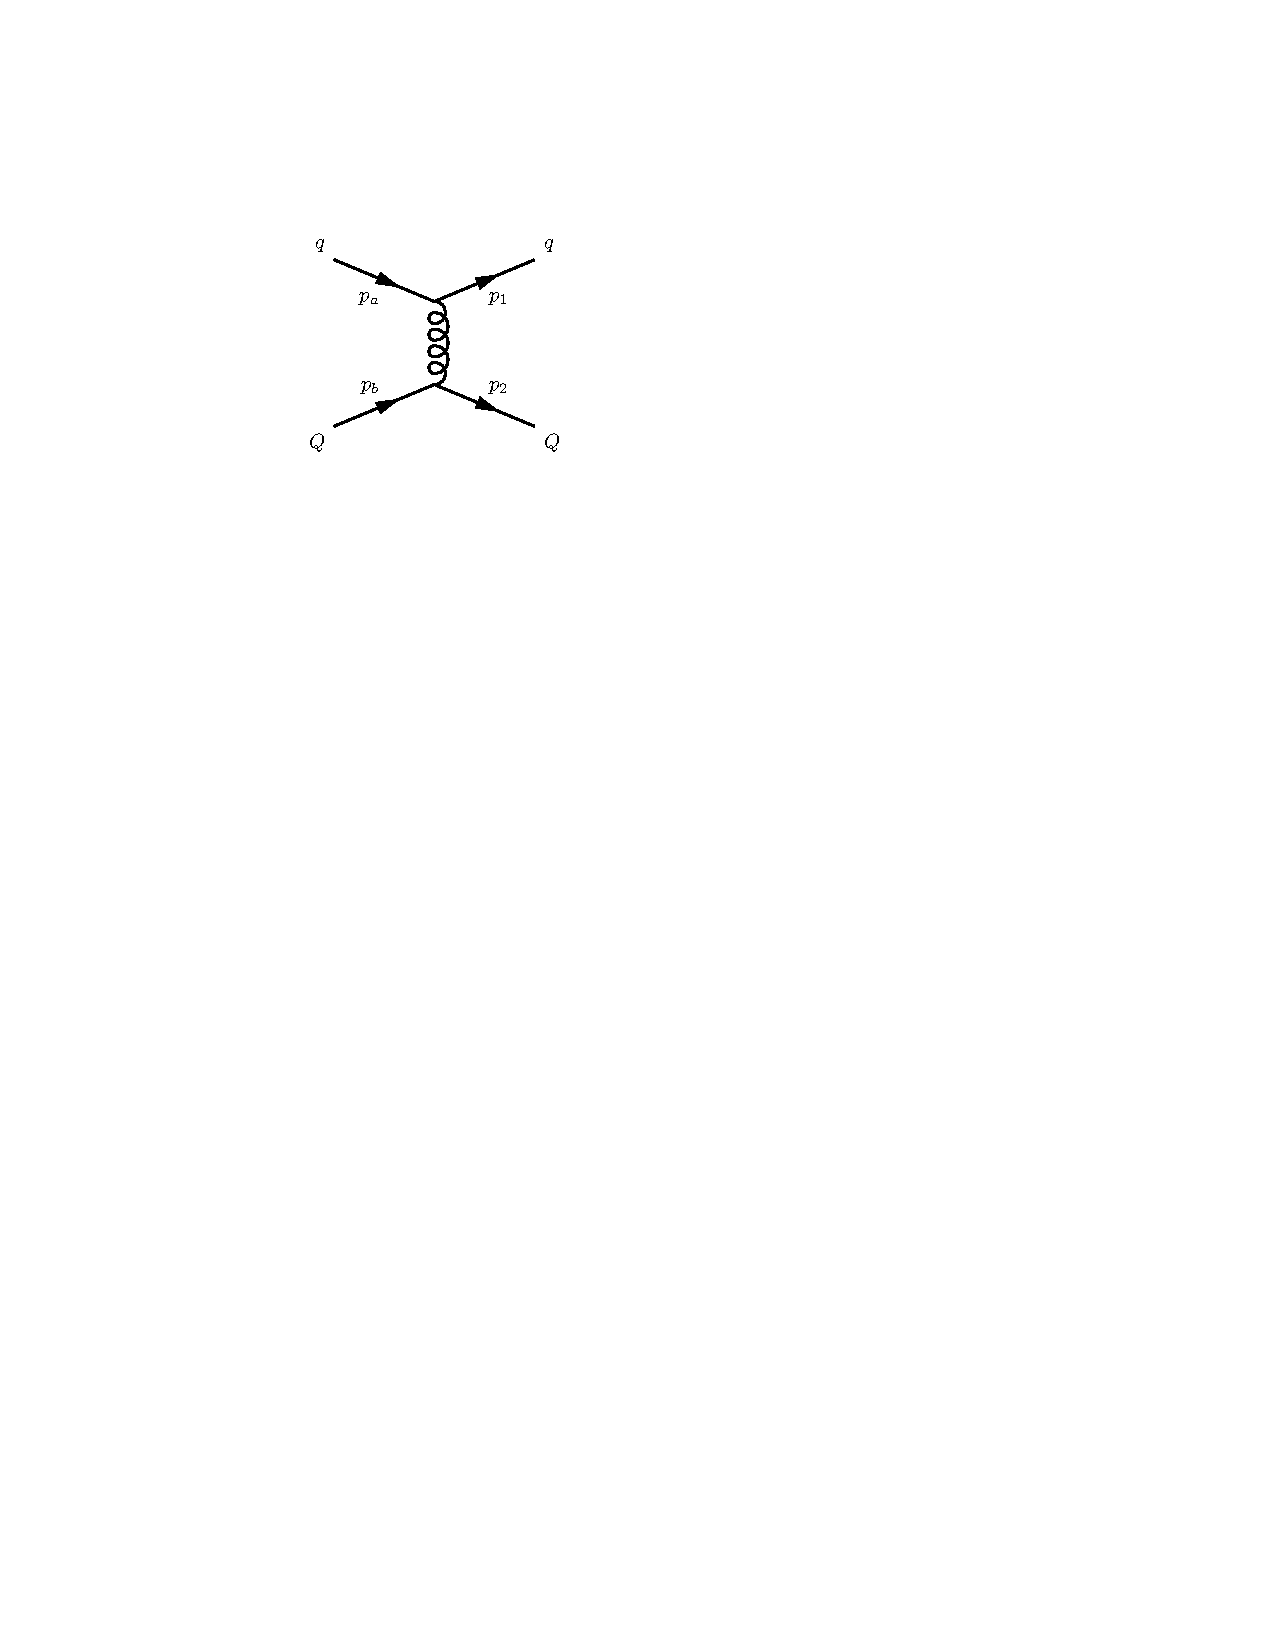
\includegraphics[width=0.35\linewidth]{TwoToTwo}
		\caption{The only diagram which contributes to $qQ\rightarrow qQ$ at leading order in $\alpha_s$.}
		\label{fig:TwoToTwo}
		\end{center}
	\end{figure}

\section{$qg$ scattering at High Energy}
	\label{sec:qg}

	We now explore the more involved case of $q^-g^+\to q^-g^+$ scattering.  At leading order this
	consists of three diagrams shown in fig.~\eqref{fig:TwoToTwo2}.  We use the following gauge
	choice for the gluon polarisations:

	\begin{align}
	\epsilon^{+*}_{2\sigma}&=\frac{\langle b|\sigma|2\rangle}{\sqrt{2}\langle b2\rangle}
	& \epsilon^{-*}_{2\sigma} &= -\frac{\langle b|\sigma|2\rangle}{\sqrt{2}[b2]} \\
	\epsilon^{+}_{b\sigma}&=-\frac{\langle b|\sigma|2\rangle}{\sqrt{2}[2b]}
	& \epsilon^{-*}_{2\sigma} &= -\frac{\langle b|\sigma|2\rangle}{\sqrt{2}\langle 2b\rangle}
	\end{align}

	For simplicity we choose to write everything in terms of negative helicity spinor-helicity brackets;
	to describe positive helicities we can use the transposition property of spinor-helicity brackets discussed
	in section~\ref{sec:SpinorHelicity}.

	\begin{figure}[h]
		\centering
		\begin{subfigure}[b]{0.3\textwidth}
			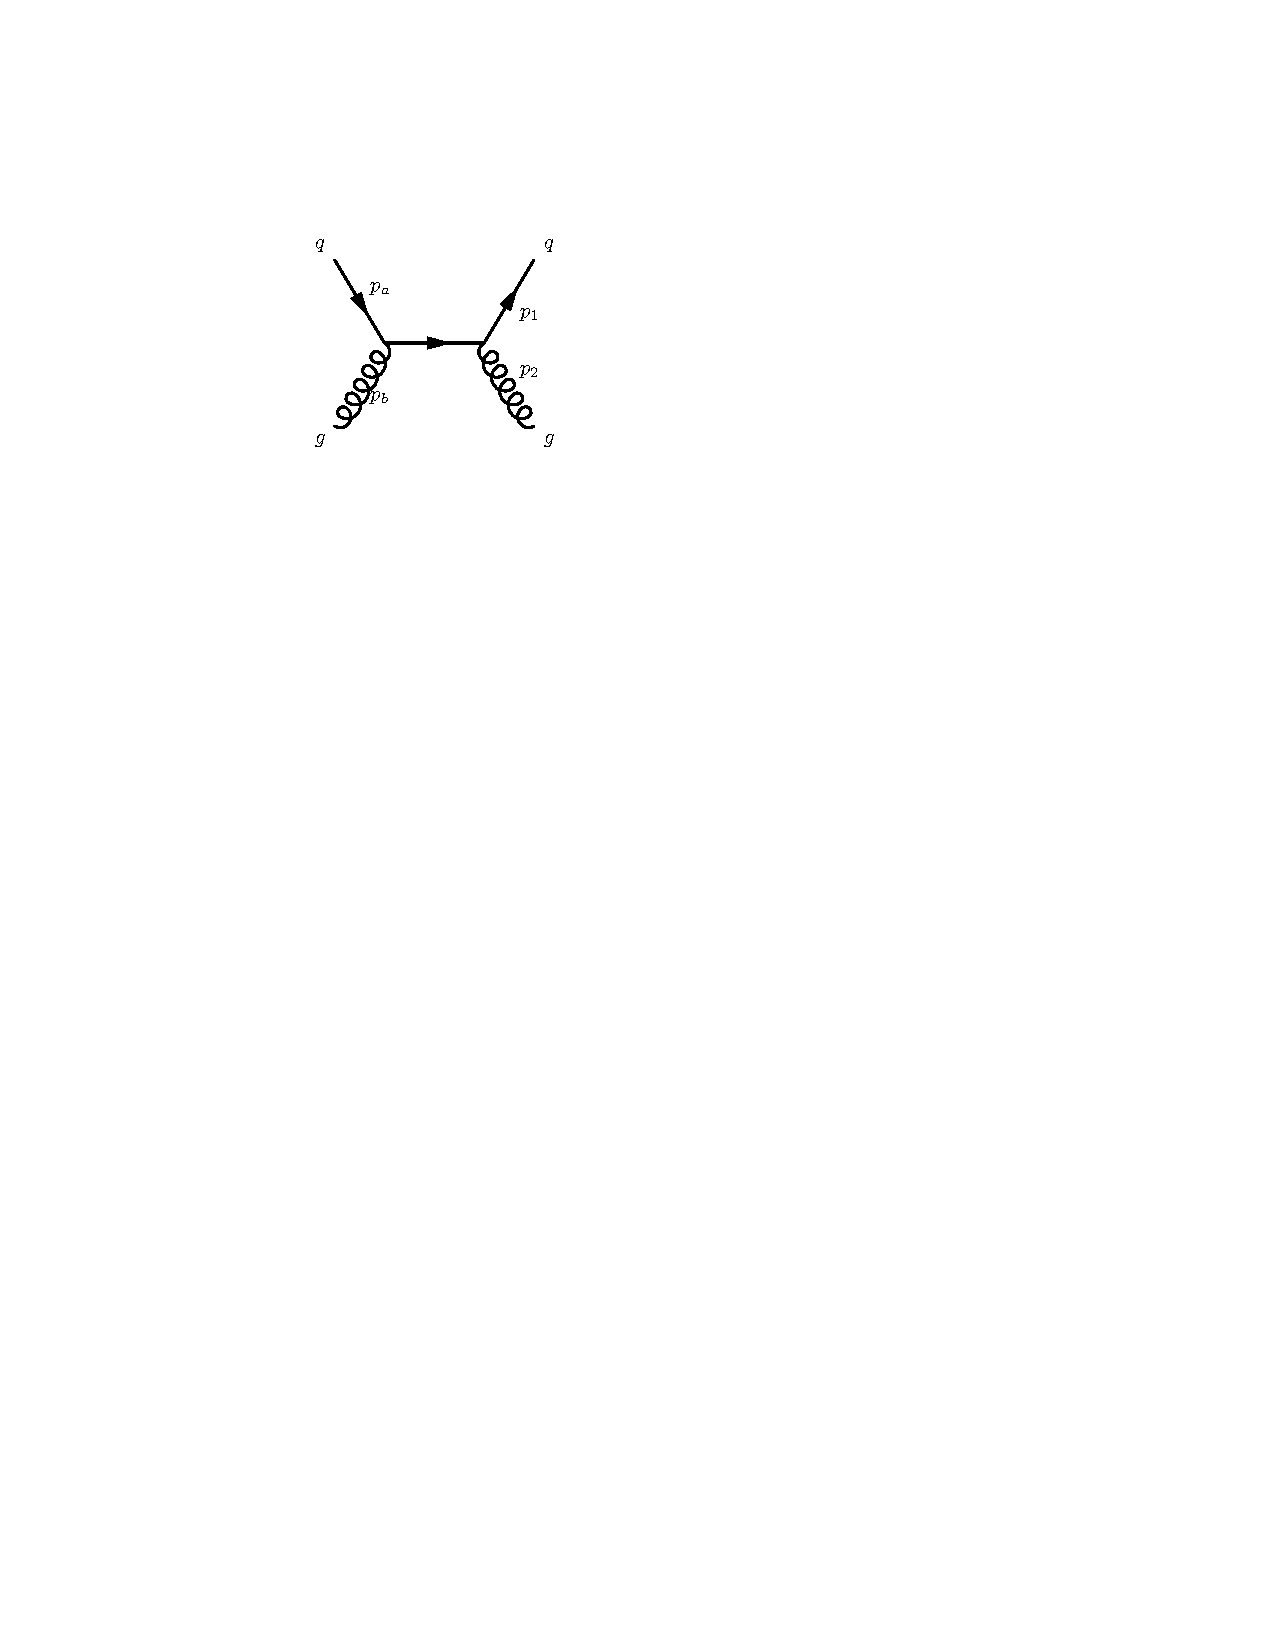
\includegraphics[width=\textwidth]{qg2qg-s}
			\caption{}
			\label{fig:qg2qg-s}
		\end{subfigure}

		\begin{subfigure}[b]{0.3\textwidth}
			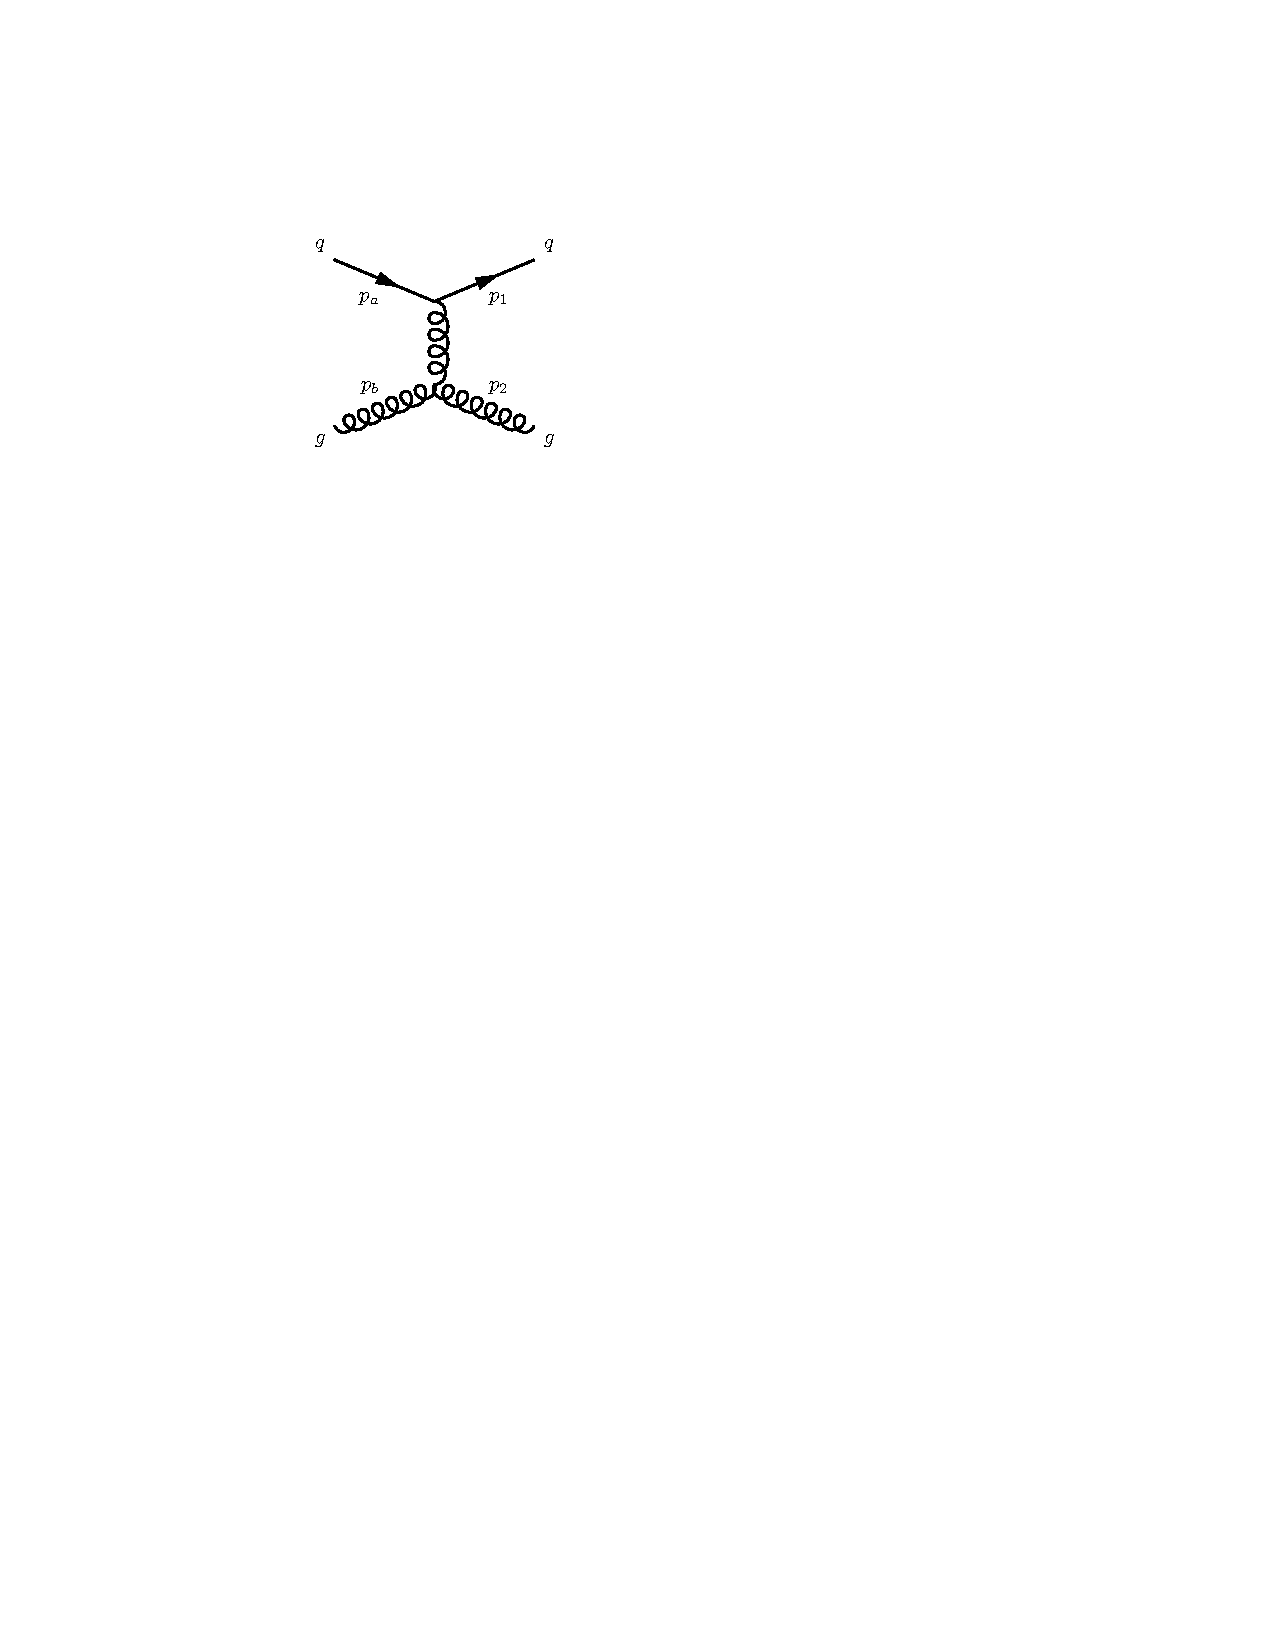
\includegraphics[width=\textwidth]{qg2qg-t}
			\caption{}
			\label{fig:qg2qg-t}
		\end{subfigure}
		~
		\begin{subfigure}[b]{0.3\textwidth}
			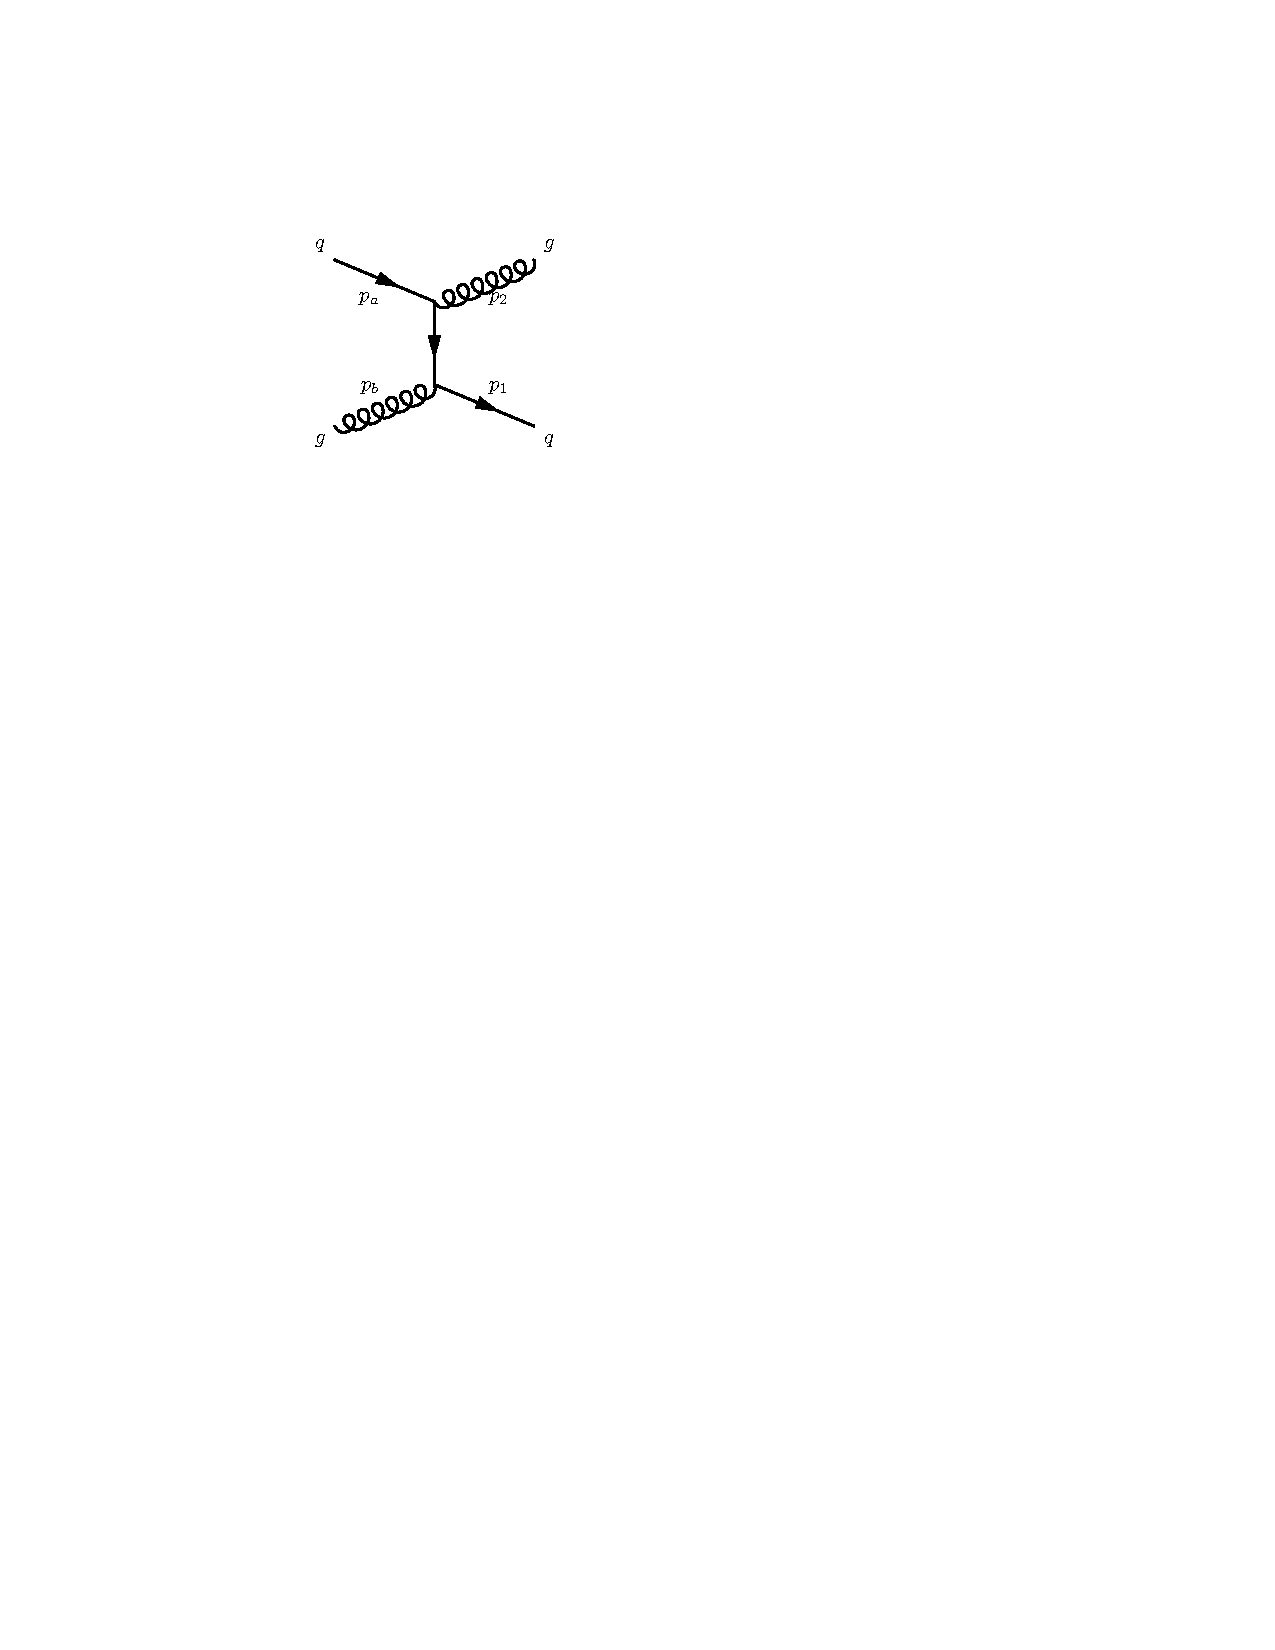
\includegraphics[width=\textwidth]{qg2qg-u}
			\caption{}
			\label{fig:qg2qg-u}
		\end{subfigure}
		\caption{The $s$, $t$ and $u$ channel diagrams contributing to $q^-g^+\to q^-g^+$ at leading
		         order in $\alpha_s$ in figures (\ref{fig:qg2qg-s}), (\ref{fig:qg2qg-t}) and (\ref{fig:qg2qg-u})
		         respectively.}
		\label{fig:TwoToTwo2}
	\end{figure}

	\subsection{$s$-channel}

		The matrix element for the $s$-diagram, shown in fig.~\eqref{fig:qg2qg-s}, is:

		\begin{align}
			\mathcal{M}_{q^-g^+\to q^-g^+, s}^{\text{LO}}=&T^b_{ae}T^2_{e1}\overline{u}^-(p_1)\left(-\frac{ig_s}{2}\gamma^\mu\right)\epsilon_\mu^{*+}(p_2)
				\frac{i(\slashed q+m)}{q^2-m^2}\left(-\frac{ig_s}{2}\gamma^\nu\right)\epsilon^+_\nu(p_b)u^-(p_a), \\
			=&-\frac{g^2_s}{4q^2}\epsilon^{*+}_{2\mu}\epsilon^+_{b\nu}\overline{u}^-_1\gamma^\mu\slashed q\gamma^\nu u^-_a,
		\end{align}

		where we have neglected the quark mass term since we are in the High Energy limit.
		The propagator has momentum $q=p_a+p_b=p_1+p_2$ and therefore:

		\begin{align}
			\mathcal{M}_{q^-g^+\to q^-g^+, s}^{\text{LO}}=&-T^b_{ae}T^2_{e1}\frac{g^2_s}{4q^2}\frac{\langle{b}|\mu|2\rangle}{\sqrt{2}\langle{b2\rangle}}
			\frac{\langle{b}|\nu|2\rangle}{\sqrt{2}[2b]}\overline{u}^-_1\gamma^\mu(\slashed{p}_a+\slashed{p}_b)\gamma^\nu u^-_a.
		\end{align}

		We use the completeness relations for $\slashed p_{a/b}$ and see that:

		\begin{equation}
			\mathcal{M}_{q^-g^+\to q^-g^+, s}^{\text{LO}}=-T^b_{ae}T^2_{e1}\frac{g^2_s}{4q^2t}[2a]\langle ab\rangle\langle{b}|\mu|2\rangle\langle{1}|\mu|a\rangle
		\end{equation}

		Using $q^2=s_{ab}=\langle ab\rangle[ba]$ and $t=\langle2b\rangle[b2]$ we have:

		\begin{equation}
		\mathcal{M}_{q^-g^+\to q^-g^+, s}^{\text{LO}}=-T^b_{ae}T^2_{e1}\frac{g^2_s}{4}\frac{[2a]\langle ab\rangle}{\langle ab\rangle[ba]
		\langle2b\rangle[b2]}\langle{b}|\mu|2\rangle\langle{1}|\mu|a\rangle.
		\label{eqn:tempLabel}
		\end{equation}

		We must now calculate explicitly the spinor product brackets using the conventions for spinors outlined in the
		previous chapter, for example:

		\begin{align}
			[2a] = &\overline{u}^+_2u^-_a=-\frac{\sqrt{p_a^+p_2^-}p_2^\perp}{|p_2^\perp|}.
		\end{align}

		After calculating the other brackets in eqn.~\eqref{eqn:tempLabel} we see:

		\begin{equation}
			\mathcal{M}_{q^-g^+\to q^-g^+, s}^{\text{LO}} = -T^b_{ae}T^2_{e1}\frac{g_s^2}{4}\sqrt{\frac{p_2^-}{p_b^-}}\frac{1}{p_2^+p_b^-} \frac{p_{2\perp}^*}{|p_{2\perp}|} \bk{b}{\mu}{2} \bk{1}{\mu}{a}
		\end{equation}

		Which can be simplified to give the final result:

		\begin{equation}
			\mathcal{M}_{q^-g^+\to q^-g^+, s}^{\text{LO}}=-T^b_{ae}T^2_{e1}\frac{g_s^2}{2\hat{t}}\sqrt{\frac{p_2^-}{p_b^-}}\frac{p_{2\perp}^*}
			{|p_{2\perp}|}\langle{b}|\mu|2\rangle\langle{1}|\mu|a\rangle
			\label{eqn:s-channel}
		\end{equation}

	\subsection{$t$-channel}

		The matrix element for the $t$-channel diagram, shown in fig.~\eqref{fig:qg2qg-t}, is:

		\begin{align}
		\begin{split}
			-i\mathcal{M}_{q^-g^+\to q^-g^+, t}^{\text{LO}} =
			&-T^e_{a1}f^{b2e}\overline{u}^-_1\Bigg(-\frac{ig_s}{2}\gamma^\mu\Bigg)\Bigg(-\frac{ig_{\mu\nu}}{q^2}\Bigg)u^-_ag_s\\
			&\Big(g_{\sigma\nu}(p_b-q)_\rho + g_{\nu\rho}(q+p_b)_\sigma - g_{\rho\sigma}(p_b+p_2)_\nu)\Big)\epsilon^{\rho *}_{2+}\epsilon^{\sigma}_{b+}\\
		\end{split}
		\end{align}

		Now using $q=p_2-p_b$ and $p_2\cdot\epsilon_2 = p_b\cdot\epsilon_b = 0$:

		\begin{align}
		\begin{split}
			-i\mathcal{M}_{q^-g^+\to q^-g^+, t}^{\text{LO}} =
		        -T^e_{a1}f^{b2e}\frac{g_s^2}{2q^2s_{2b}}\left(\overline{u}^-_1\gamma^{\nu}u^-_a\right)\left(\overline{u}^-_b\gamma^{\rho}u^-_2\right)\left(\overline{u}^-_b\gamma^{\sigma}u^-_2\right)\\
			\Big(2g_{\sigma\nu}p_{b\rho} + 2g_{\nu\rho}p_{2\sigma} - g_{\rho\sigma}(p_b+p_2)_\nu\Big),
		\end{split}
		\end{align}

		which cancels completely and therefore:

		\begin{equation}
			\mathcal{M}_{q^-g^+\to q^-g^+, t}^{\text{LO}}=0,
			\label{eqn:t-channel}
		\end{equation}

		in this gauge.

	\subsection{$u$-channel}

		The matrix element for the $u$-diagram, shown in fig.~\eqref{fig:qg2qg-u}, is:

		\begin{equation}
			\begin{split}
			-i\mathcal{M}_{q^-g^+\to q^-g^+, u}^{\text{LO}} &= T^2_{ae}T^b_{e1}\overline{u}^-(p_1)\left(-\frac{ig_s}{2}\gamma^\mu\right)
			\frac{i(\slashed q+mc)}{q^2-m^2c^2}\left(-\frac{ig_s}{2}\gamma^\nu\right)u^-(p_a)\epsilon_\mu^{*+}(p_b)\epsilon^+_\nu(p_2)\\
			\mathcal{A}_u &= \frac{g_s^2}{4q^2}\overline{u}^-_1\gamma^\mu\slashed q\gamma^\nu u^-_a\epsilon^{+*}_{b\mu}\epsilon^*_{2\nu}\\
			&= \frac{g_s^2}{8q^2s_{2b}}\langle b|\mu|2\rangle\langle b|\nu|1\rangle\overline{u}^-_1\gamma^\mu(\slashed{p}_a-\slashed{p}_2)\gamma^\nu u^-_a\\
			\end{split}
		\end{equation}

		Where we have used $q=p_a-p_2$.  By direct comparison with the procedure used for the $s$-channel we can see the result will be:

		\begin{equation}
		\mathcal{M}_{q^-g^+\to q^-g^+, u}^{\text{LO}}=
		T^2_{ae}T^b_{e1}\frac{g_s^2}{2\hat{t}}\sqrt{\frac{p_b^-}{p_2^-}}\frac{p^*_{2\perp}}{|p_{2\perp}|}\langle{b}|\mu|2\rangle\langle{1}|\mu|a\rangle.
		\label{eqn:u-channel}
		\end{equation}

		The total total matrix element is given by the sum of eqs.~\eqref{eqn:s-channel},~\eqref{eqn:t-channel} and~\eqref{eqn:u-channel} which is:

		\begin{equation}
			\mathcal{M}_{q^-g^+\to q^-g^+}^{\text{LO}}=
			\frac{g_s^2}{2}\frac{p_{2\perp}^*}{|p_{2\perp}|}\left(T^2_{ae}T^b_{e1}\sqrt{\frac{p_b^-}{p_2^-}}-T^b_{ae}T^2_{e1}
			\sqrt{\frac{p_2^-}{p_b^-}}\right)\frac{\langle{b}|\mu|2\rangle\langle{1}|\mu|a\rangle}{\hat{t}},
			\label{eqn:fullsum}
		\end{equation}

		We also see that eqn.~\eqref{eqn:fullsum} has the same spinor-helicity brackets contracted as eqn.~\eqref{eqn:similarBrackets}
		and so the dominant behaviour of $q^-g^+\to q^-g^+$ in the high energy limit is $\frac{s}{t}$.
		In the High Energy limit we have $p_b^-\thicksim p_2^-$ and so eqn.~\eqref{eqn:fullsum} could be simplified
		further to:

		\begin{equation}
			\mathcal{M}_{q^-g^+\to q^-g^+}^{\text{LO}}=i\frac{g_s^2}{2}\frac{p_{2\perp}^*}{|p_{2\perp}|}f^{2bc}T^c_{a1}
			\frac{\langle{b}|\mu|2\rangle\langle{1}|\mu|a\rangle}{\hat{t}}.
			\label{eqn:fullsum2}
		\end{equation}

		which is identical to the result found in the previous $qQ\rightarrow qQ$ calculation (save for a phase which cancels
		at the amplitude squared level). The kinematics of eqn.~\eqref{eqn:fullsum} are exactly in the form of two `currents' contracted as
		seen in section~\ref{sec:qQScat}.  We have:

		\begin{equation}
			\mathcal{M}_{qg\to qg}^{\text{LO}} = \frac{C_A}{C_f} \mathcal{M}_{qQ\to qQ}^{\text{LO}},
		\end{equation}

		in the High Energy limit. In practice we actually choose \emph{not} to take the High Energy limit to obtain
		eqn.~\eqref{eqn:fullsum2} so as to approximate as little as possible.  Even without this extra approximation
		eqn.~\eqref{eqn:fullsum} is still exactly the form of a $t$-channel gluon exchange as seen in
		eqn.~\eqref{eqn:similarBrackets}.

		In section~\ref{sec:HEJ} we will return this result and the results of section~\ref{sec:qQScat} and discuss how,
		despite their simplicity, they can be used to construct very general approximate forms for matrix elements which
		could otherwise not be evaluated

\section{$qQ$-scattering at High Energy (at NLO)}
	\label{sub:HE22_NLO}

	Before we continue on to look at how we might add extra real emissions to high energy matrix
	elements we briefly look at higher order (in $\alpha_s$) corrections to the process we studied in
	section~\ref{sec:qQScat}.  So far we have seen the leading order processes with a $t$-channel
	exchange are enhanced but in eqn.~\eqref{eqn:schematicExpn} we sketched out a form for
	the perturbative expansion which also had enhanced contributions at higher order orders.

	Here we continue on from section~\ref{sec:qQScat} and calculate the virtual diagrams which contribute
	a leading logarithm for $qQ\to qQ$ at next-to-leading in $\alpha_s$~\cite{sabioThesis,DelDuca:1995hf}.

	We might expect that the next-to-leading order diagrams with the maximal number of $t$-channel exchanges
	will give the greatest enhancement and, indeed, this turns out to be the case.  These diagrams are shown
	for the case of $qQ\rightarrow qQ$ in fig.~\eqref{fig:NLO-leadingContrib}.  We can rule out the other
	virtual diagrams which contribute at this order since they will contain (anti-)quark propagators along
	the $p_{a/1}$ or $p_{b/2}$ lines and in the high energy limit these will be suppressed.

	These diagrams in fig.~\eqref{fig:NLO-leadingContrib} can be elegantly computed by using the `Cutkosky
	rules' which are used to relate two sub-diagrams to the imaginary part of a higher order diagram through
	the Optical theorem.  This can be seen very quickly since the scattering matrix, $S$, must be unitary i.e.
	$S^\dagger S=1$.  If we write this instead in terms of the the transition matrix, $T$, defined by $S=1+iT$
	then we immediately have that

	\begin{equation}
		-i(T - T^\dagger) = T^\dagger T.
	\end{equation}

	The left hand side of which can be written as twice the imaginary part of $T$.  If we now let
	$T$ represent the transition from some initial state $|i\rangle$ to some final state
	$|f\rangle$ then we can write this as:

	\begin{equation}
		2i\text{Im}(\bk{i}{T}{f}) =  \sum_{p}\bk{i}{T^\dagger}{p}\bk{p}{T}{f},
	\end{equation}

	where we have inserted a sum over a complete set of states $|p\rangle$.  Pictorially we `cut' propagators
	by forcing them on-shell with delta functions and inserting a complete set of states.

	For example the uncrossed amplitude in fig.~\eqref{fig:NLO-uncrossed},
	$\mathcal{M}_{qQ\rightarrow qQ}^{\text{NLO, II}}$, may be expressed as a combination of
	two copies of the amplitude arising from fig.~\eqref{fig:TwoToTwo}:

	\begin{figure}[tpb]

		\centering
		\captionsetup[subfigure]{oneside, margin={-1.5cm, 0cm, 0cm}}
		\begin{subfigure}[b]{0.48\textwidth}
			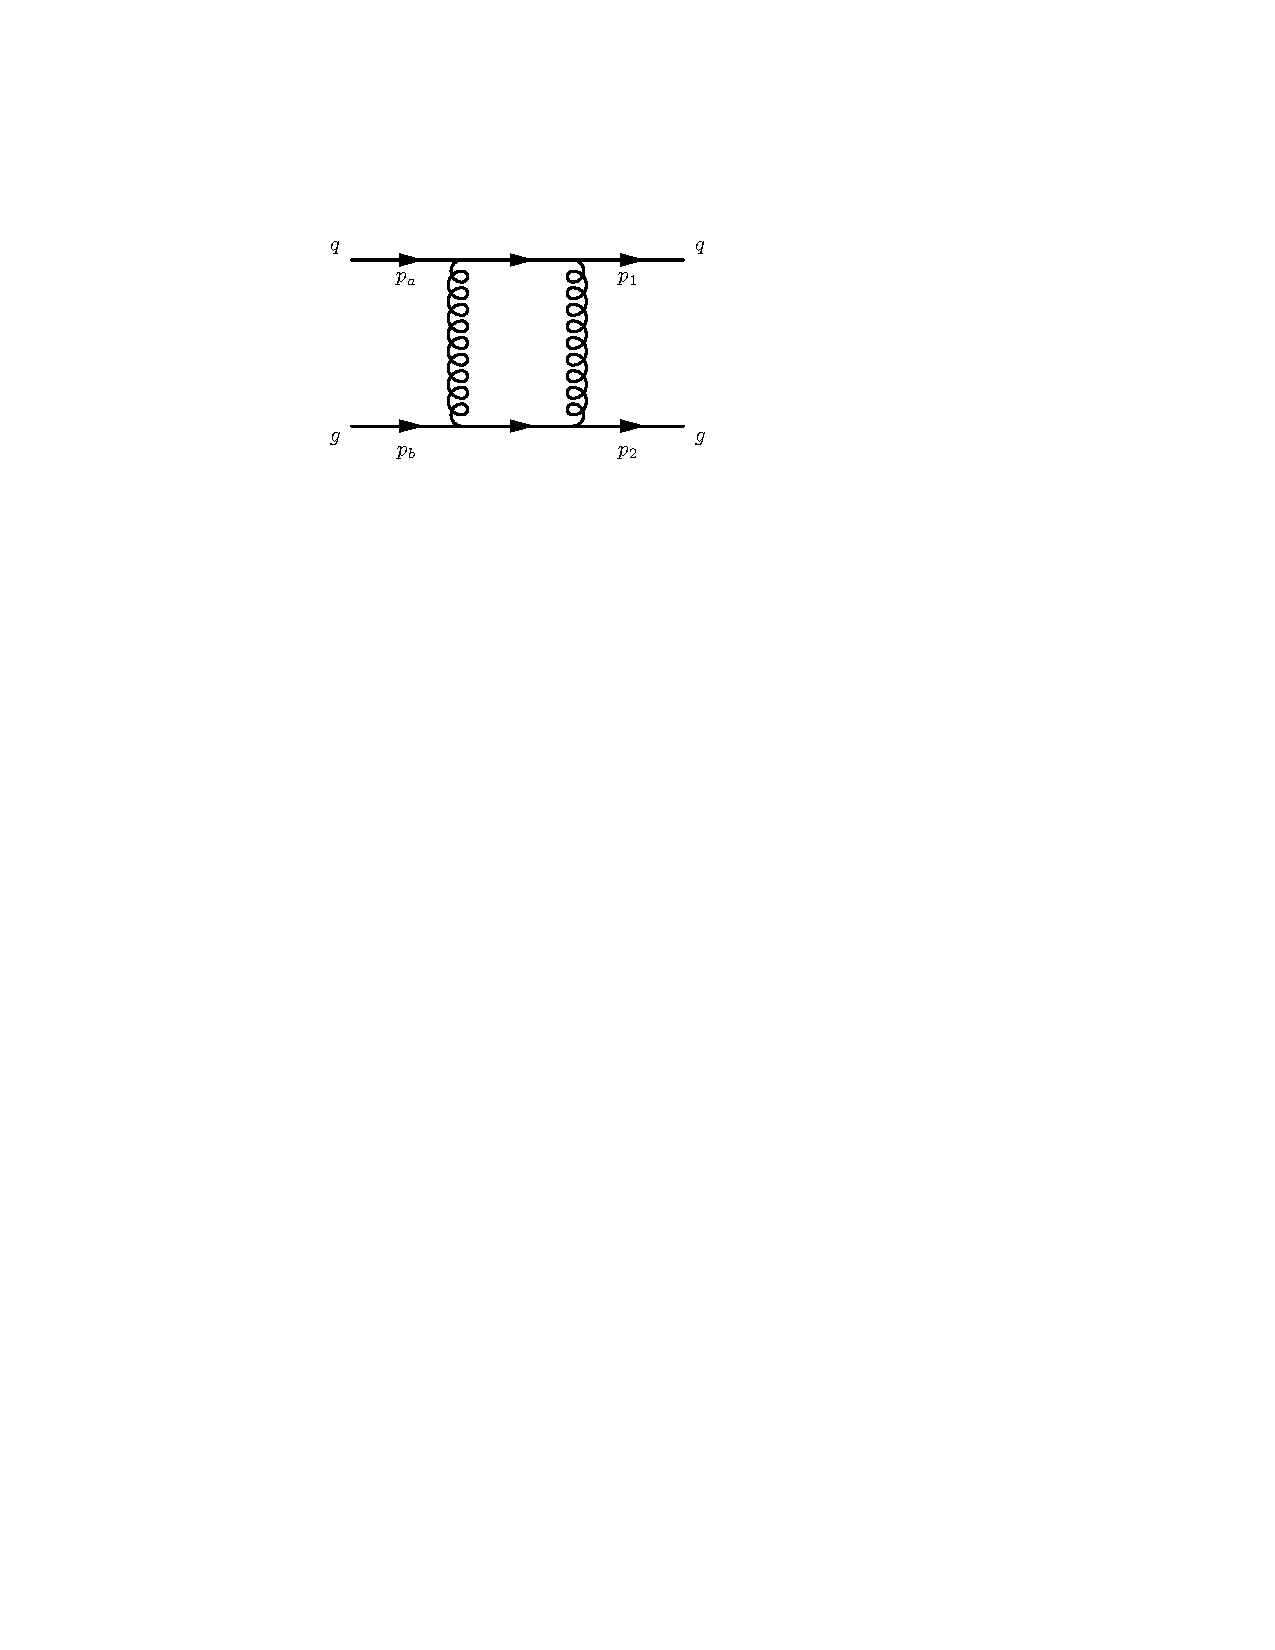
\includegraphics[width=0.8\textwidth]{NLO-uncrossed}
			\caption{}
			\label{fig:NLO-uncrossed}
		\end{subfigure}
		\begin{subfigure}[b]{0.48\textwidth}
			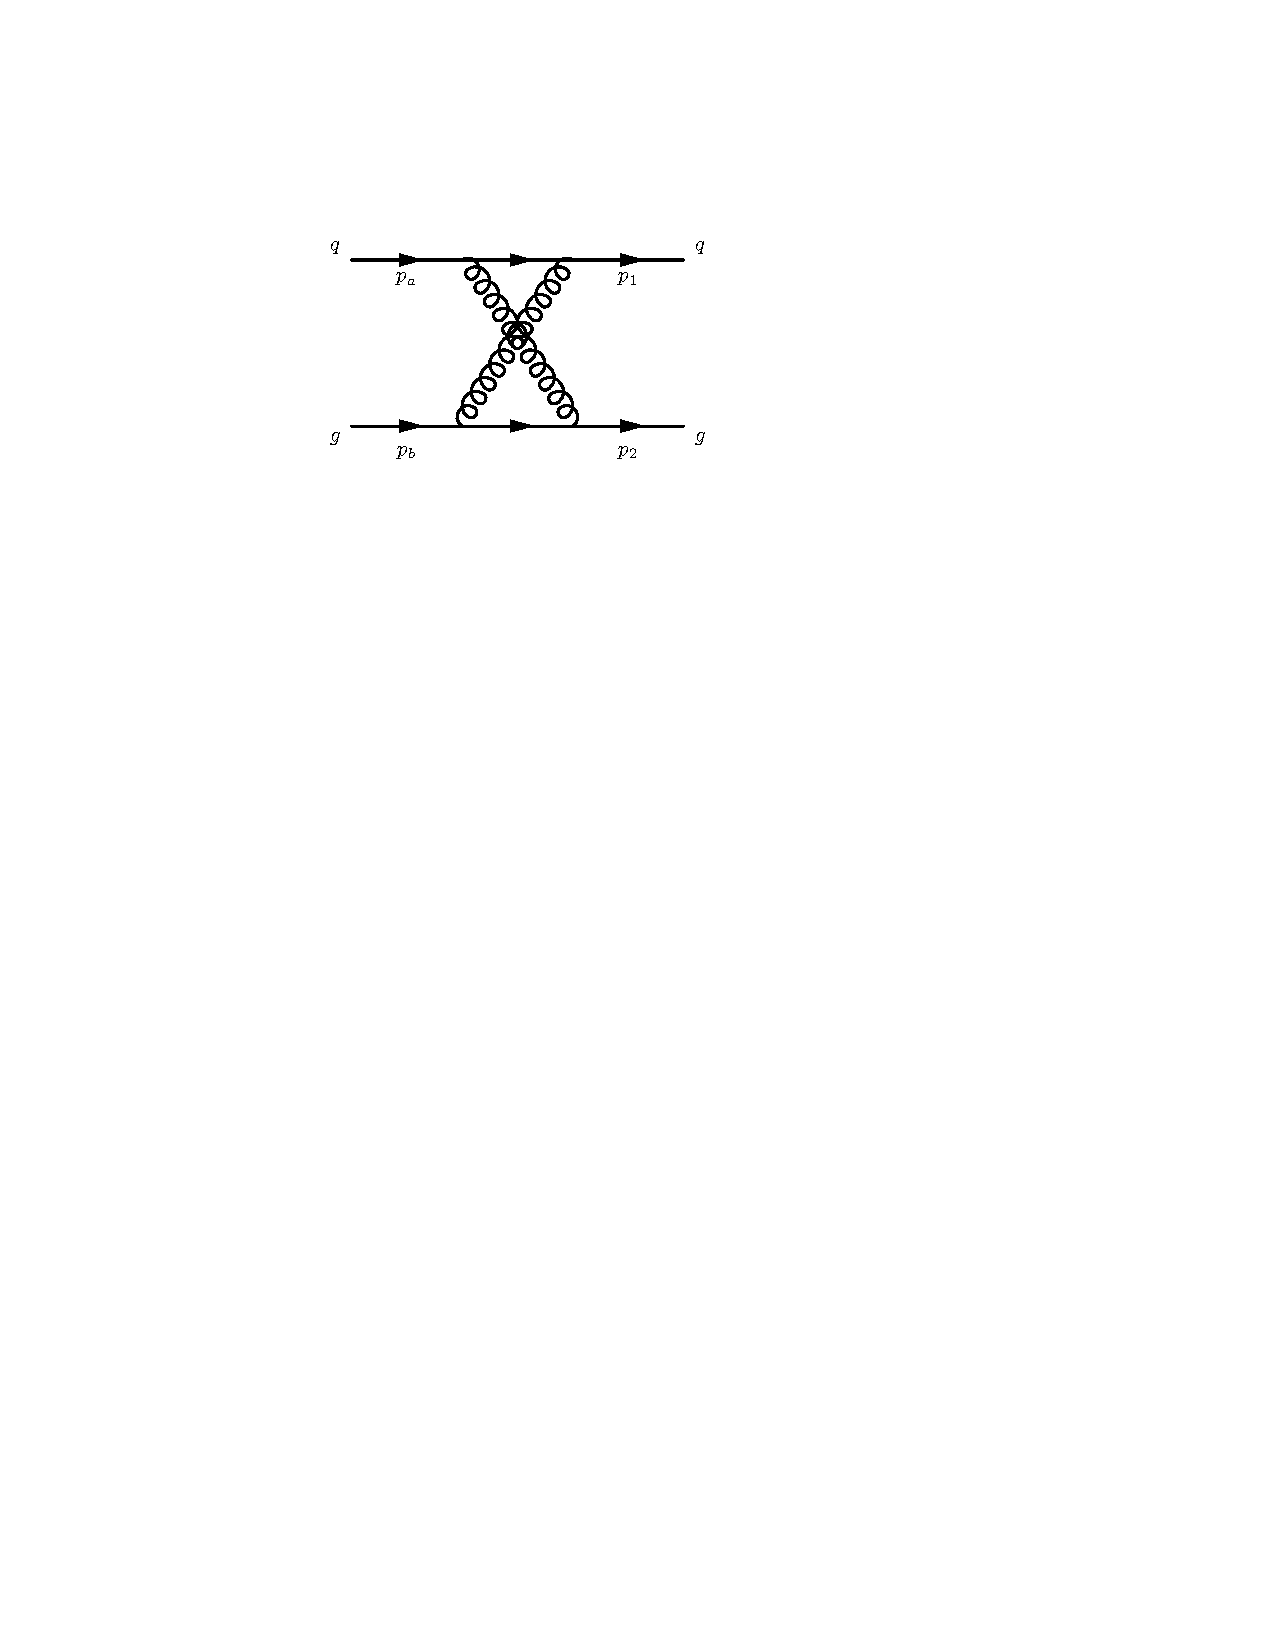
\includegraphics[width=0.8\textwidth]{NLO-crossed}
			\caption{}
			\label{fig:NLO-crossed}
		\end{subfigure}
		\caption{The leading logarithmic contributions to $qg\rightarrow qg$ at NLO.  The uncrossed
			         diagram, $\mathcal{M}_{qQ\rightarrow qQ}^{\text{NLO}, II}$, shown in (a) exchanges
			         two gluons in the $t$ channel and the crossed diagram,
			         $\mathcal{M}_{qQ\rightarrow qQ}^{\text{NLO}, X}$, case (b) exchanges two gluons
			         in the $u$ channel and is related to (a) (up to a colour factor) via a crossing
			         symmetry}
		\label{fig:NLO-leadingContrib}
	\end{figure}

	\begin{equation}
		\mathcal{M}_{q^-Q^-\rightarrow q^-Q^-}^{\text{LO}} =
		-g_s^2T^d_{1a}T^d_{2b}\frac{\bk{1}{\mu}{a}\cdot\bk{2}{\mu}{b}}{t},
	\end{equation}

	as follows:

	\begin{align}
		2\text{Im}\Big(\mathcal{M}_{qQ\rightarrow qQ}^{\text{NLO, II}}\Big) =
		\frac{1}{(2\pi)^2}\int &d^4k\text{ }\delta((p_a-k)^2)
		\delta((p_b+k)^2)\\ &\mathcal{M}_{q^-Q^-\rightarrow q^-Q^-}^{\text{LO}}(k)
		\mathcal{M}_{q^-Q^-\rightarrow q^-Q^-}^{\dagger\text{LO}}(k-q),
	\end{align}

	where $\text{Im}(\cdot)$ denotes the imaginary part, $k$ is the loop momentum, $q$ is the momentum
	transfer and $\dagger$ denotes Hermitian conjugation.  The sum a complete of states here
	corresponds to integrating over all possible momenta flowing around the loop. In the High Energy
	limit we can perform the integration to give:

	\begin{equation}
		\text{Im}\Big(\mathcal{M}_{qQ\rightarrow qQ}^{\text{NLO, II}}\Big) =
		4\alpha_s^2 s\text{ }\mathcal{C}_1(T^a,T^b)
		\int \frac{dk_{\perp}}{k_{\perp}(k_{\perp} - q_{\perp})},
	\end{equation}

	where $\mathcal{C}_1(T^a,T^b)$ is the colour factor for the diagram in fig.~\eqref{fig:NLO-uncrossed}
	and $k_{\perp}$ is the transverse component of $k$.  We can now relate the
	imaginary part of the amplitude to the full amplitude by conjecturing that the amplitude will be
	logarithmically enhanced as follows:

	\begin{align}
	\begin{split}
		\mathcal{M}_{qQ\rightarrow qQ}^{\text{NLO, II}} =
		&\text{Re}(\mathcal{M}_{qQ\rightarrow qQ}^{\text{NLO, II}}) +
		i\text{Im}(\mathcal{M}_{qQ\rightarrow qQ}^{\text{NLO, II}}),
	\end{split}
	\end{align}

	and defining $\widetilde{\mathcal{M}}_{qQ\rightarrow qQ}^{\text{NLO, II}}$ as the leading
	logarithmic coefficient of the matrix element:

	\begin{align}
	\begin{split}
		\mathcal{M}_{qQ\rightarrow qQ}^{\text{NLO, II}} =&\widetilde{\mathcal{M}}_{qQ\rightarrow qQ}^{\text{NLO, II}}\ln\frac{s}{t} + \text{sub-leading}\\
		=&\widetilde{\mathcal{M}}_{qQ\rightarrow qQ}^{\text{NLO, II}}
		\left(\ln\left|\frac{s}{t}\right| -i\pi\right)+ \text{sub-leading},
		\label{eqn:rAndI}
	\end{split}
	\end{align}

	where we have used that $\frac{s}{t} < 0$.  Comparing real and imaginary parts of eqn.~\eqref{eqn:rAndI}
	and assuming that $\widetilde{\mathcal{M}}_{qQ\rightarrow qQ}^{\text{NLO, II}}$ is real we see that:

	\begin{equation}
		\text{Re}\Big(\mathcal{M}_{qQ\rightarrow qQ}^{\text{NLO, II}}\Big) =
		-\frac{1}{\pi}\text{Im}\Big(\mathcal{M}_{qQ\rightarrow qQ}^{\text{NLO, II}}\Big)
	\end{equation}

	and we can therefore reconstruct the real part of the amplitude as:

	\begin{equation}
		\text{Re}\Big(\mathcal{M}_{qQ\rightarrow qQ}^{\text{NLO, II}}\Big) =
		-\frac{4\alpha_s^2s}{\pi} \mathcal{C}_1(T^a,T^b)
		\ln\left|\frac{s}{t}\right|\int \frac{dk_{\perp}}{k_{\perp}(k_{\perp} - q_{\perp})}.
		\label{eqn:uncrossedNLOcontrib}
	\end{equation}

	The crossed-diagram,~\eqref{fig:NLO-crossed}, also contributes a leading logarithmic piece and is related to
	eqn.~\eqref{fig:NLO-uncrossed} by a crossing symmetry and so we simply replace $u$ with $s$ in eqn.
	\eqref{eqn:uncrossedNLOcontrib} and calculate a new colour factor, $\mathcal{C}_2(T^a,T^b)$:

	\begin{equation}
		\text{Re}\Big(\mathcal{M}_{qQ\rightarrow qQ}^{\text{NLO, X}}\Big) =
		-\frac{4\alpha_s^2u}{\pi} \mathcal{C}_2(T^a,T^b)
		\ln\left|\frac{u}{t}\right| \int \frac{dk_{\perp}}{k_{\perp}(k_{\perp} - q_{\perp})}.
		\label{eqn:crossedNLOcontrib}
	\end{equation}

	But in the high energy limit $s\sim -u$ (this is clear from eqn.~\eqref{eqn:mandel2}) and so we
	can combine these terms and express the leading logarithmic part of the NLO correction in terms of the leading order
	result:

	\begin{equation}
		\mathcal{M}_{qQ\rightarrow qQ}^{\text{NLO}} = \frac{3\alpha_s}{\pi^2}
		\hat{\alpha}(q)\ln\left|\frac{s}{t}\right|
		\mathcal{M}_{qQ\rightarrow qQ}^{\text{LO}},
		\label{eqn:enhancedNLO}
	\end{equation}

	where:

	\begin{equation}
		\hat{\alpha}(q) = \int dk_{\perp}\frac{q_{\perp}^2}{k_{\perp}(k_{\perp} - q_{\perp})}.
		\label{eqn:lipDiverge}
	\end{equation}

	From eqn.~\eqref{eqn:enhancedNLO} we can see the logarithmic enhancement explicitly; there is still
	a suppression from the inclusion of an extra factor of $\alpha_s$ with respect to the leading
	order term but as we have seen previously the logarithm is related to the kinematics of the final
	state - namely - the rapidity gap between the outgoing quarks $p_1$ and $p_2$ and this can be large enough to compensate
	for the smallness of $\alpha_s$.  Eqn.~\eqref{eqn:lipDiverge} will clearly diverge when we
	come to integrate over the soft region (where $k_\perp$ is very small).  This divergence
	will be treated, i.e. regularised and explicitly shown to cancel, in chapter~\ref{chap:Zs}.

\section{$t$-channel Dominance}
	\label{sec:tChannel}

	In what follows we construct high multiplicity matrix elements by approximating the full result
	by the contraction of two currents and a number of effective vertices.  This choice allows us
	to construct matrix elements which contains the leading logarithms.\\
	As a simple example we consider the production of 4 exclusive jets in the High Energy limit.
	We present a brief argument for precisely which diagrams contribute these leading logarithms.
	Although heuristic it is sufficient to motivate the construction of high multiplicity amplitudes from
	$t$-channel gluon exchanges with the understanding that any other diagrams will be formally sub-leading.
	Fig.~\eqref{fig:quadJets} shows three diagrams which all contribute at leading order in $\alpha_s$;
	fig.~\eqref{fig:quadJets1} has three gluons exchanged in the $t$-channel and so its amplitude will
	have propagator terms which goes like:

	\begin{equation}
		\mathcal{M}_{\text{(a)}}\sim\frac{1}{(p_a - p_1)^2(p_a - p_1 - p_2)^2(p_a - p_1 - p_2 - p_3)^2},
		\label{eqn:inPlace}
	\end{equation}

	By contrast figs.~\eqref{fig:quadJets2} and~\eqref{fig:quadJets3} will
	have, in place of~\eqref{eqn:inPlace}:

	\begin{align}
		\mathcal{M}_{\text{(b)}}\sim\frac{\slashed p_a - \slashed p_1}
		{(p_a - p_1)^2(p_a - p_1 - p_2)^2(p_a - p_1 - p_2 - p_3)^2},\\
		\intertext{and,}
		\mathcal{M}_{\text{(c)}}\sim\frac{(\slashed p_a - \slashed p_1)(\slashed p_4 - \slashed p_b)}
		{(p_a - p_1)^2(p_a - p_1 - p_2)^2(p_a - p_1 - p_2 - p_3)^2},
	\end{align}

	\begin{figure}[bt]

		\centering

		\begin{subfigure}[b]{0.31\textwidth}
			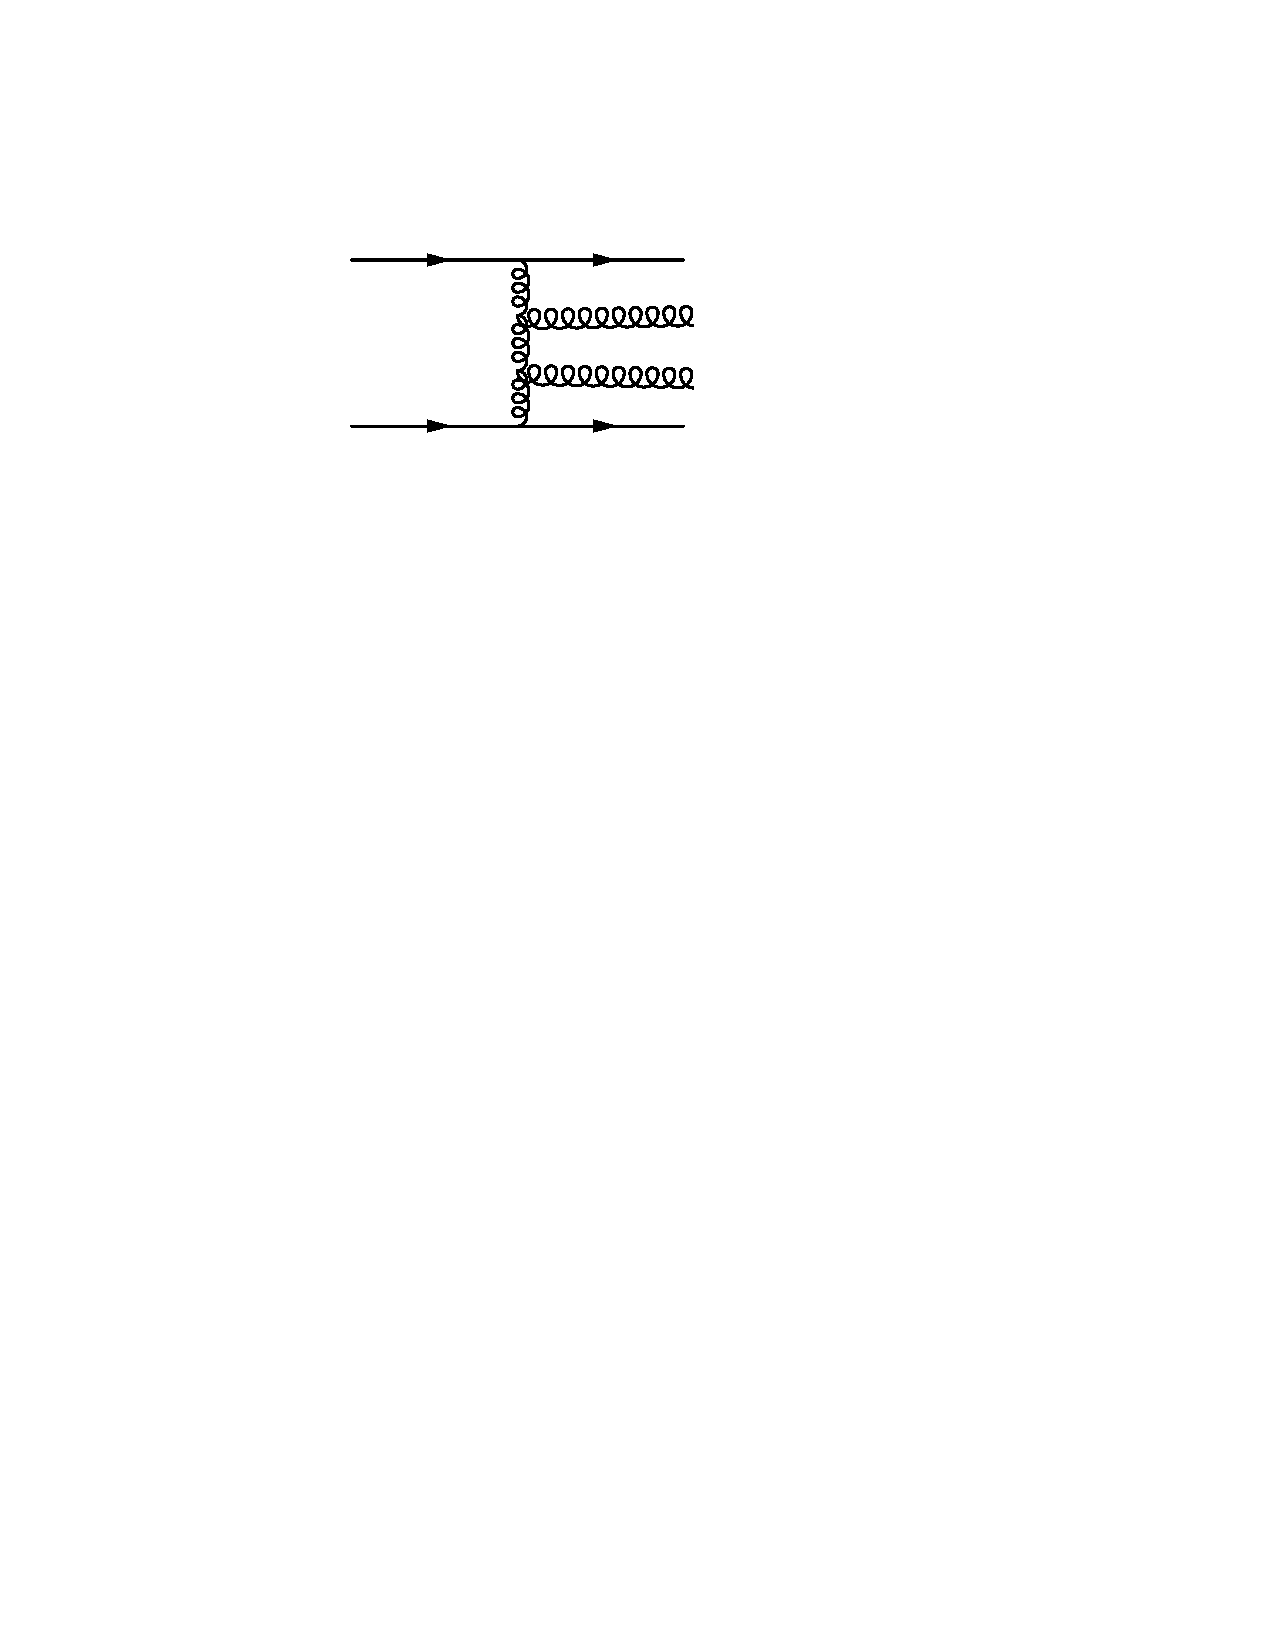
\includegraphics[width=\textwidth, height=0.7\textwidth]{quadJets1}
			\caption{}
			\label{fig:quadJets1}
		\end{subfigure}
		\begin{subfigure}[b]{0.31\textwidth}
			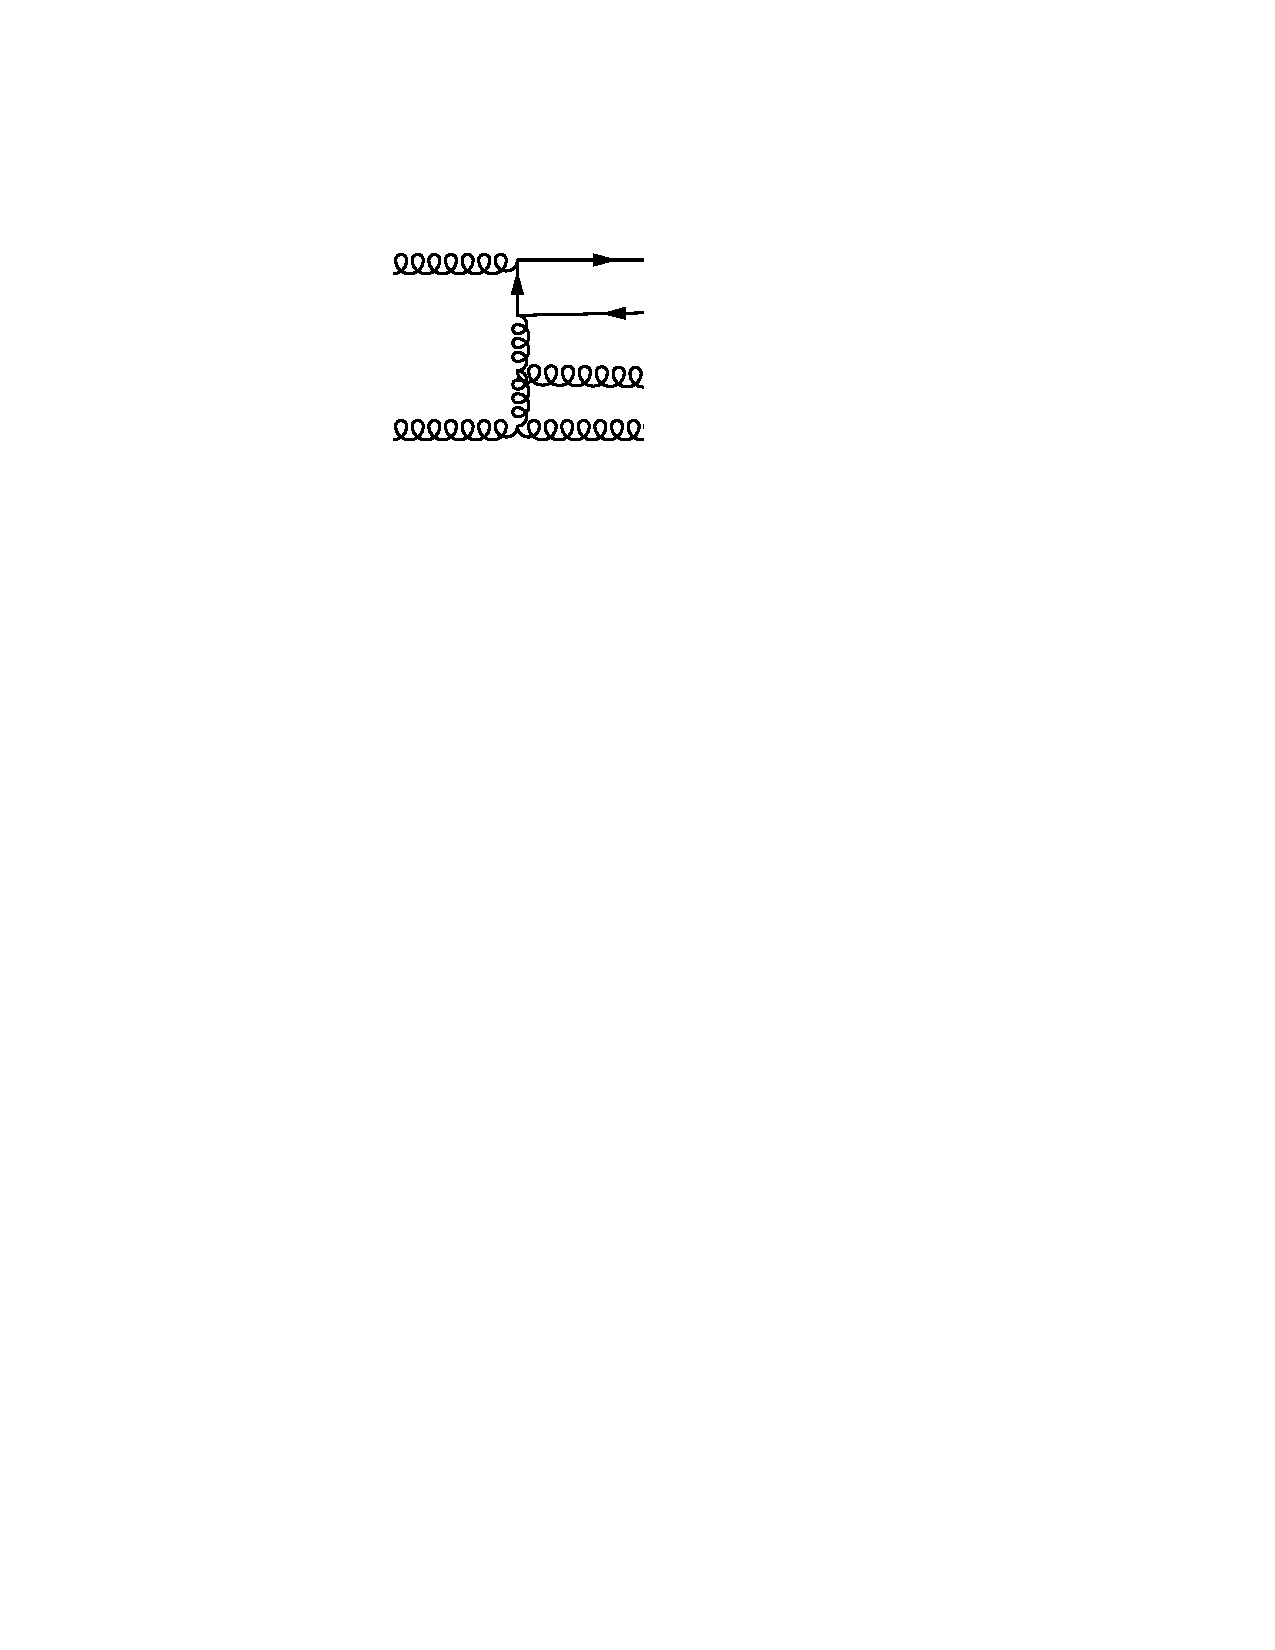
\includegraphics[width=\textwidth, height=0.7\textwidth]{quadJets2}
			\caption{}
			\label{fig:quadJets2}
		\end{subfigure}
		\begin{subfigure}[b]{0.31\textwidth}
			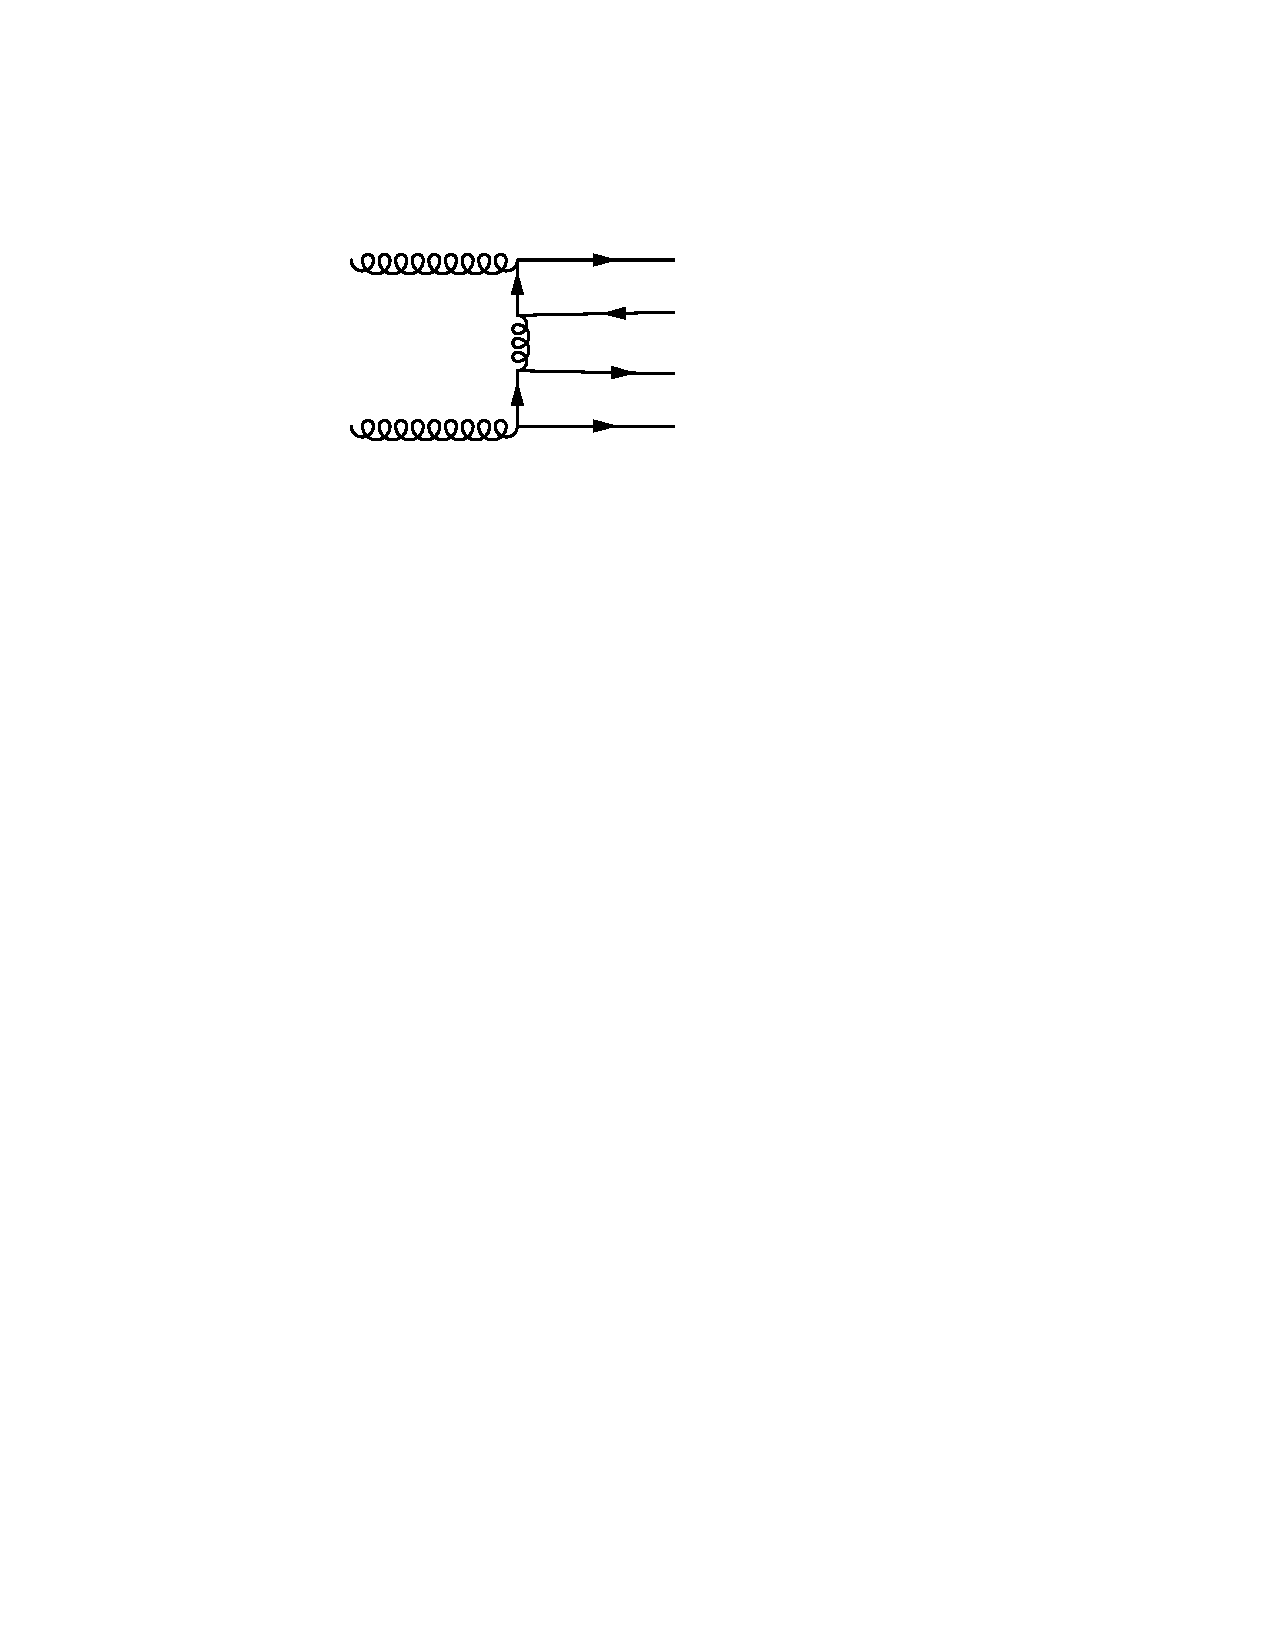
\includegraphics[width=\textwidth, height=0.7\textwidth]{quadJets3}
			\caption{}
			\label{fig:quadJets3}
		\end{subfigure}

		\caption{Three processes contributing to exclusive four jet production. (a) has the
		maximum number of gluons exchanged in the $t$-channels (three) and will dominate in the High
		Energy limit, (b) and (c) only have two and one gluon which can reggeise.  As such as we move
		from (a) to (c) we will lose powers of large logarithms but maintain the same power of
		$\alpha_s$ and therefore we can reasonably approximate quad-jet production by neglecting
		(b) and (c) in the High Energy limit.}
		\label{fig:quadJets}
	\end{figure}

	respectively.  Since in the High
	Energy limit we have $p_a\sim p_1$ and $p_b\sim p_4$ it is clear that $\mathcal{M}_{\text{(b)}}$
	and $\mathcal{M}_{\text{(c)}}$ will be suppressed with respect to $\mathcal{M}_{\text{(a)}}$. We call
	the configurations with a maximal number of gluons exchanged in the $t$-channels an `FKL' configuration;
	For example fig.~\eqref{fig:quadJets1} is an FKL configuration while fig.~\eqref{fig:quadJets2} and fig.
	\eqref{fig:quadJets3} are `non-FKL' configurations.

	A formal argument for which processes dominate in this limit was given by Fadin and Lipatov
	\cite{Kuraev:1976ge,Balitsky:1978ic}.  They found that, in the High Energy limit, scattering
	amplitudes scaled in the same way as was predicted by Regge theory.  This states that in the
	large invariant mass region a $2\to n$ matrix element has a limiting behaviour determined by
	the maximum spin of any particle which could be exchanged in the $t$-channels between final
	state partons neighbouring in rapidity.  We can then find the scaling of a process, for example
	$qg\to qg$, in particular regions of phase space where either $y_g\gg y_q$ or $y_q\gg y_g$ simply
	by drawing the associated colour connection diagrams for it.  This is shown in~\eqref{fig:colorConns}.
	Since when we have $y_g\gg y_q$ it is only possible to exchange a colour singlet (with spin one half)
	the cross-section will be dominated by the region where $y_q\gg y_g$.  The case for $2\to n$ is similar
	with the limiting behaviour of the matrix element given by

	\begin{equation}
		\mathcal{M}^{\text{HE}}_{2\to n}\sim s_{12}^{\omega_1}\cdots s_{(n-1)n}^{\omega_{(n-1)}}.
		\label{eqn:reggeScaling}
	\end{equation}

	Eqn.~\eqref{eqn:reggeScaling} now makes the previous discussion regarding figs.~\eqref{fig:quadJets}
	formally clear since fig.~\eqref{fig:quadJets1} will scale like:

	\begin{equation}
		\mathcal{M}^{\text{HE}}_{2\to 4} \sim s_{12}s_{23}s_{34},
	\end{equation}

	in the High Energy limit while figs.~\eqref{fig:quadJets2} and~\eqref{fig:quadJets3} will scale
	like:

	\begin{align}
	\begin{split}
		\mathcal{M}^{\text{HE}}_{2\to 4} \sim s_{12}^{\nicefrac{1}{2}}s_{23}s_{34},\\
	\end{split}
	\end{align}

	and,

	\begin{align}
	\begin{split}
		\mathcal{M}^{\text{HE}}_{2\to 4} \sim s_{12}^{\nicefrac{1}{2}}s_{23}s_{34}^{\nicefrac{1}{2}},
	\end{split}
	\end{align}

	respectively.  Since $s_{ij}$ are all large here, the processes with a (anti)quark exchanged
	in the $t$-channel will be highly suppressed relative to fig.~\eqref{fig:quadJets1}.

	\begin{figure}[bth]
		\begin{center}
		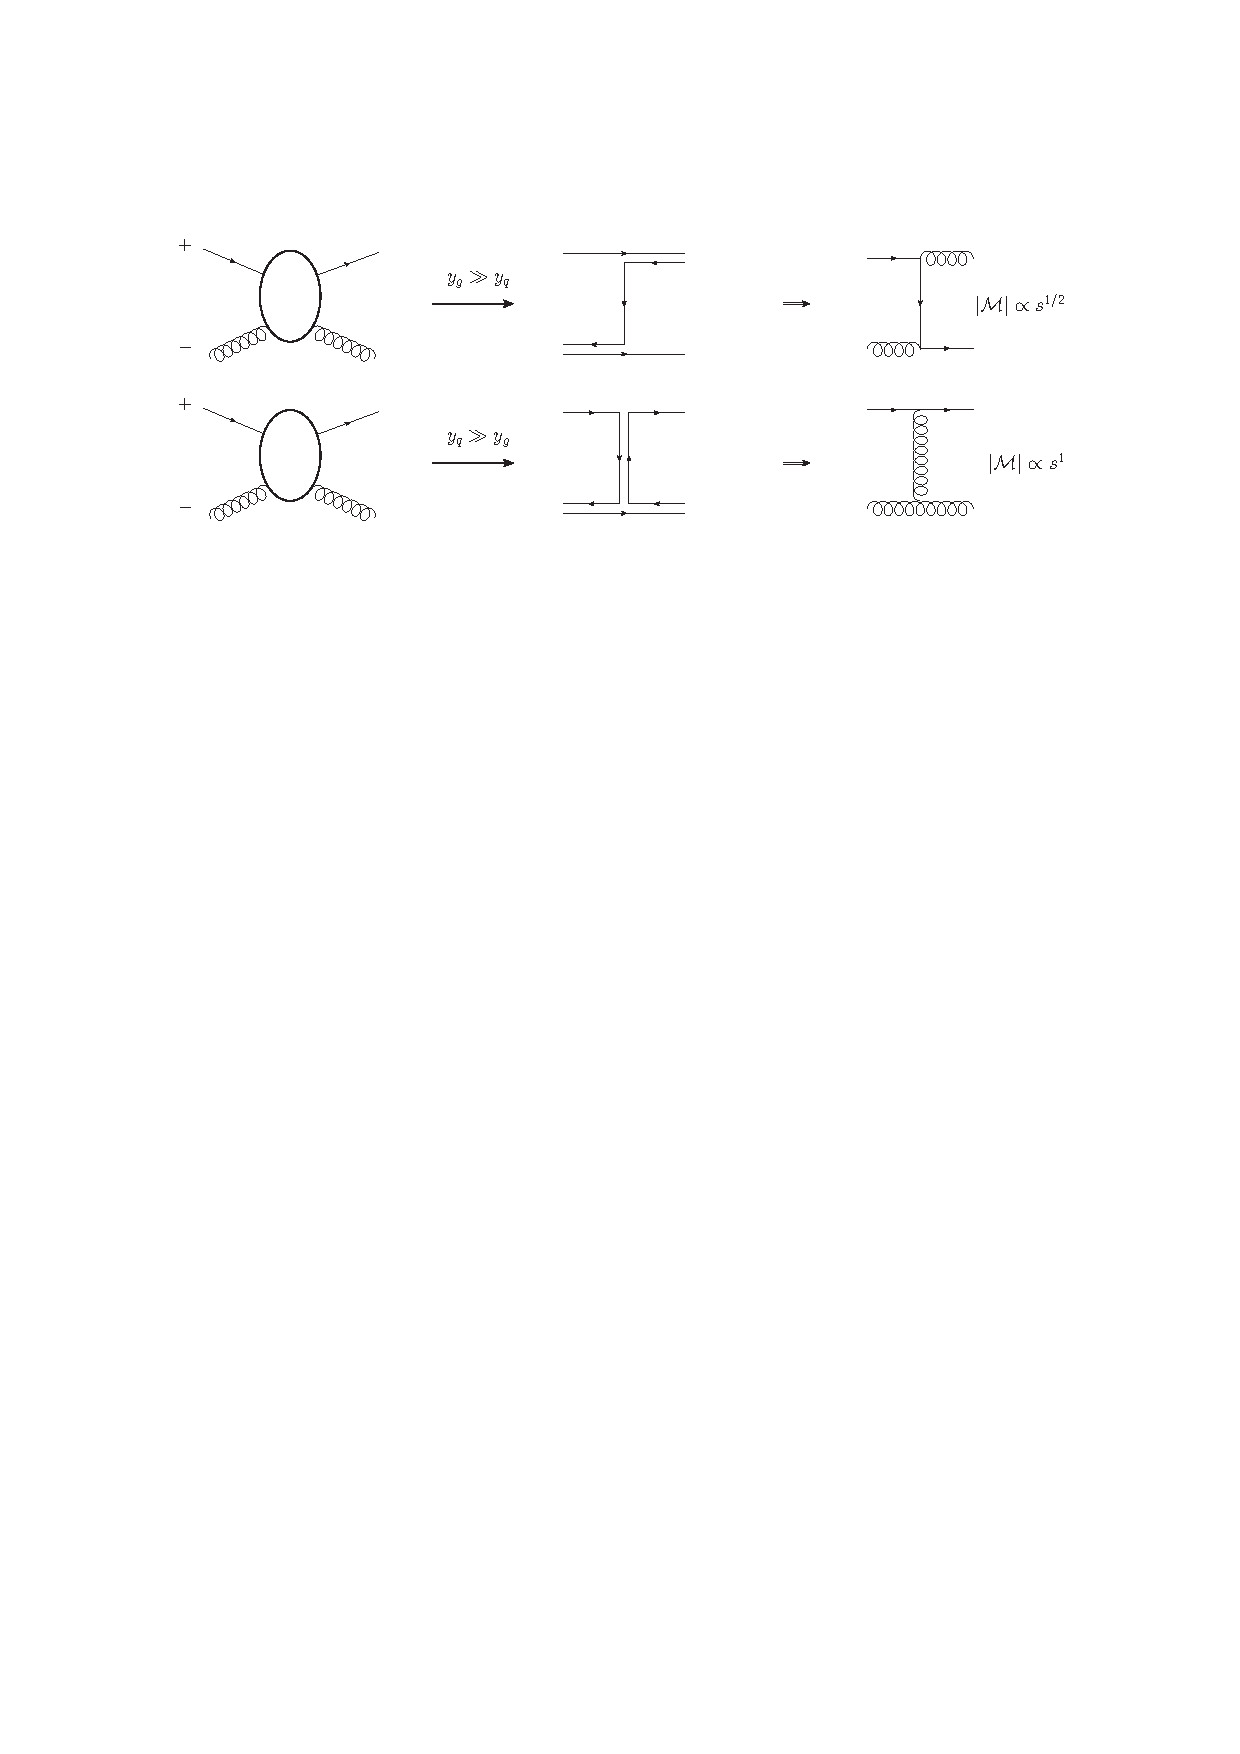
\includegraphics[width=1.0\linewidth]{ColourConns}
		\caption{The limiting behaviour of $qg\to qg$ in the regions of phase space where
		either $y_g\gg y_q$ or $y_q\gg y_g$.  The intermediate diagrams indicate the flow
		of colour through the process.}
		\label{fig:colorConns}
		\end{center}
	\end{figure}

	To further illustrate this we can look at the various processes contributing to the exclusive two
	jet cross-section.  Table~\ref{tab:LOatHE} shows several examples of parton level
	processes and their exact leading order matrix elements~\cite{pinkBook}.  We can see clearly
	from this that any process which can proceed via a $t$-channel gluon exchange has a term
	proportional to $s^2/t^2$ which will dominate in the High Energy limit; for
	example $q\bar{Q}\to q\bar{Q}$ can only go via a $t$-channel diagram.
	Conversely, processes in which a $t$-channel gluon diagram can not contribute are
	suppressed in this limit.  For example $q\bar{q}\to Q\bar{Q}$ can only proceed via an
	$s$-channel gluon and we can see that in the limit $s\to\infty$ and keeping $t$ finite it's matrix
	element tends to $-\nicefrac{4}{9}$ (since $s\sim-u$ in the High Energy limit).  Processes
	like $gg\to gg$ have diagrams with and without the exchange we are interested in
	and, as such, only some of the terms from the exact leading order matrix element
	contribute - but they do still contribute.

	\begin{table}[hbt!]
		\begin{center}
		\begin{tabular}{c | c }
		Process                 & $\nicefrac{1}{g^4}|\bar{\mathcal{M}}|^2$ \\ \hline
		$qQ\to qQ$              & $\frac{4}{9}\frac{s^2 + u^2}{t^2}$       \\
		$q\bar{Q}\to q\bar{Q}$  & $\frac{4}{9}\frac{s^2 + u^2}{t^2}$       \\
		$qq\to qq$              & $\frac{4}{9}\left(\frac{s^2 + u^2}{t^2} + \frac{s^2 + t^2}{u^2}\right) - \frac{8}{27}\frac{s^2}{ut}$\\
		$q\bar{q}\to Q\bar{Q}$  & $\frac{4}{9}\frac{t^2 + u^2}{s^2}$       \\
		$gg\to gg$              & $\frac{9}{2}\left(3-\frac{tu}{s^2}-\frac{su}{t^2}-\frac{st}{u^2}\right)$\\
		\end{tabular}
		\caption{Some examples of $2\to2$ leading order matrix elements which contribute to the
		two jet exclusive cross-section.}
		\label{tab:LOatHE}
		\end{center}
	\end{table}

\section{Effective Vertices For Real Emissions}
	\label{sec:effectiveVertices}

	In order to generalise what we have done so far to higher multiplicity scattering events we begin
	by considering $qQ\rightarrow qQg$ in the high energy limit.  The five diagrams which contribute at
	leading order are illustrated in fig.~\eqref{fig:2To3}.  The diagram
	where the extra gluon is emitted from the $t$-channel gluon is given by:

	\begin{figure}[t]
		\begin{center}
		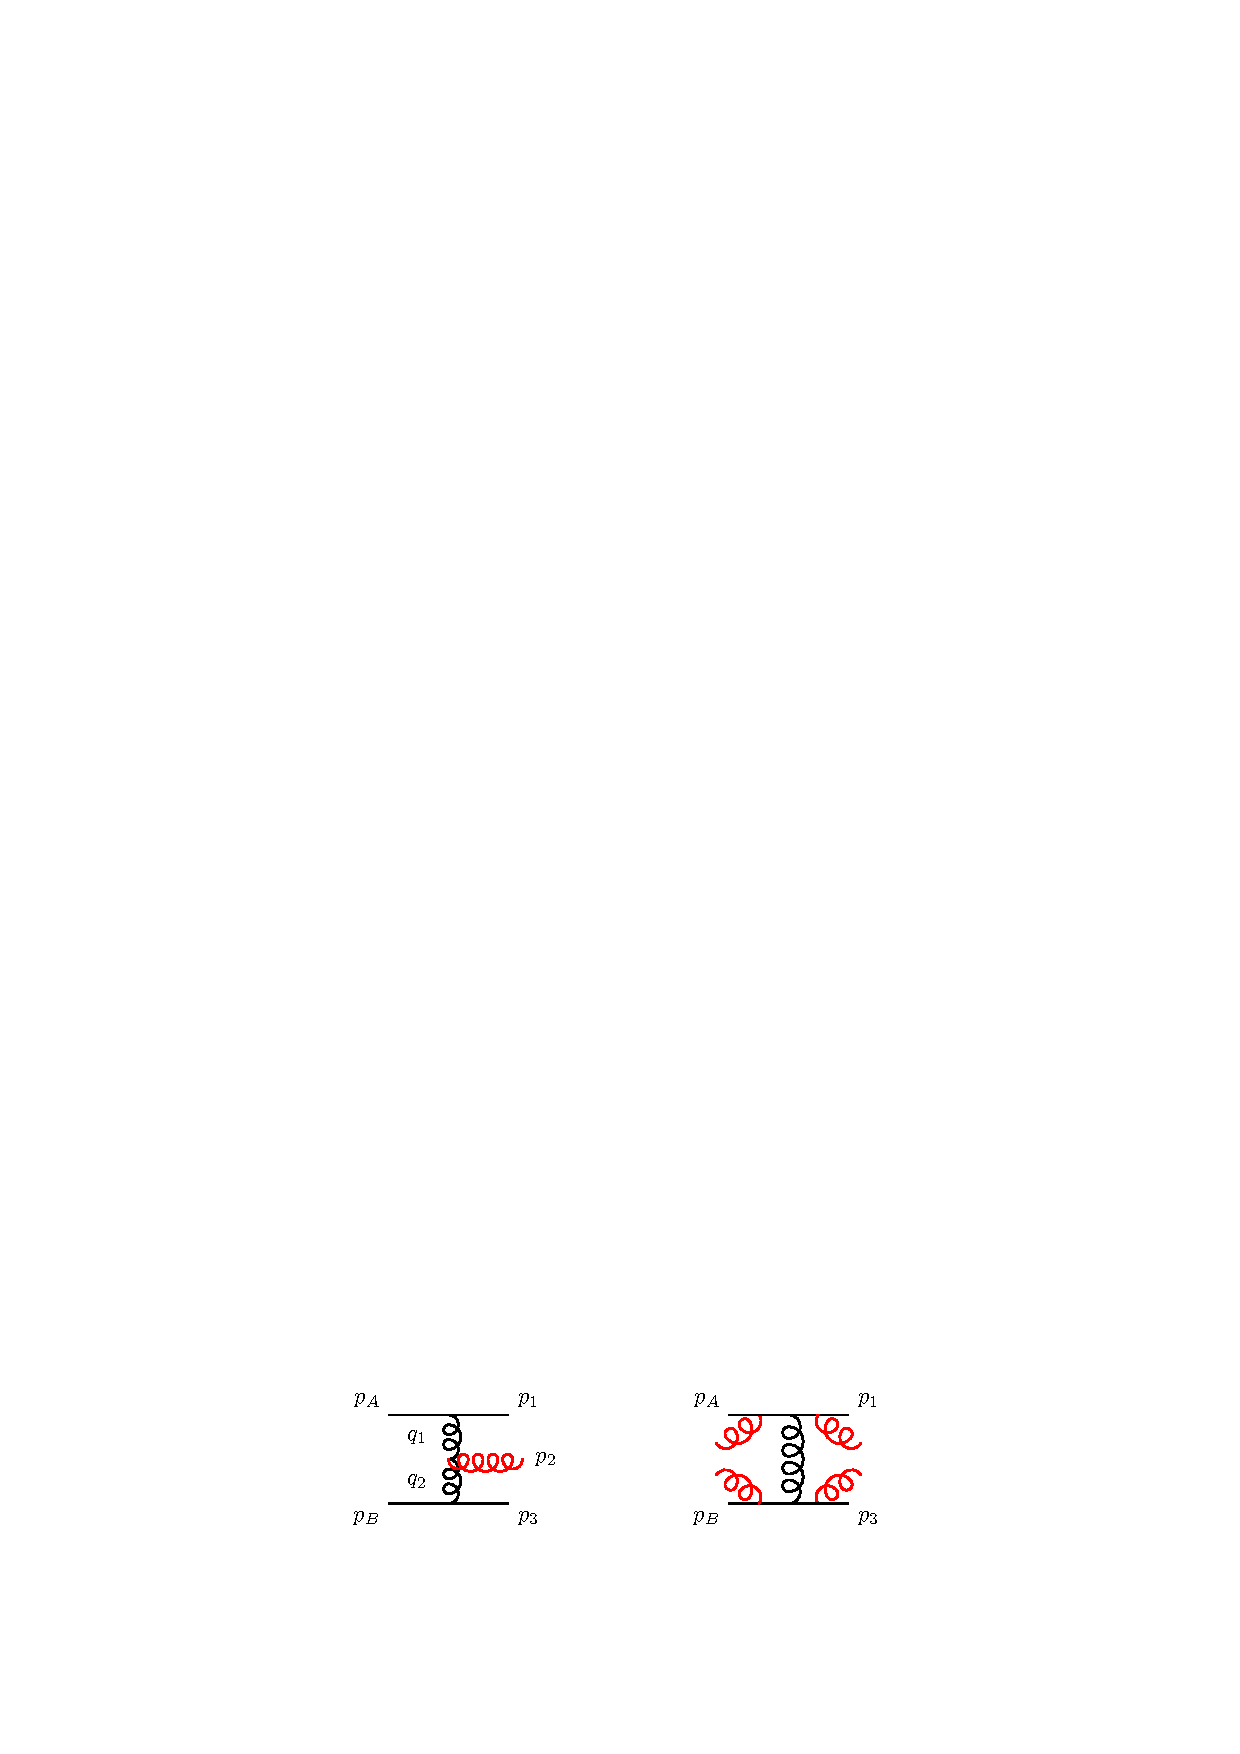
\includegraphics[width=0.7\linewidth]{2To3}
		\caption{The 5 possible emission sites of extra QCD radiation in $qQ\rightarrow qQ$.
		Fig. from \cite{Andersen:2009nu}.}
		\label{fig:2To3}
		\end{center}
	\end{figure}

	\begin{align}
	\begin{split}
		\mathcal{M}_{t\text{-channel}} = &-\frac{g_s^3}{t_{a1}t_{b2}}f^{i2j}T^i_{1a}T^j_{3b}\bk{1}{\rho}{a}\bk{3}{\mu}{b}
		\epsilon^*_{2\nu}\\&\left(2p_2^\mu g^{\nu\rho} - 2p_2^\rho g^{\mu\nu} - (q_1 + q_2)^\nu g^{\mu\rho} \right),
		\label{eqn:mtchannel}
	\end{split}
	\end{align}

	and the remaining four diagrams are:

	\begin{align}
	\begin{split}
	    \mathcal{M}_{\text{Eik.}} = (ig_s)^3 \epsilon_{2\nu} \Bigg(
	     &T^2_{1i}T^d_{ia}T^d_{3b}\ \frac{2p_1^\nu\bk{1}{\mu}{a} + \bk{1}{\nu}{2}\bk{2}{\mu}{a}} {s_{12}t_{b3}} \bk{3}{\mu}{b} \\
	    +&T^d_{1i}T^2_{ia}T^d_{3b}\ \frac{2p_a^\nu\bk{1}{\mu}{a} - \bk{1}{\mu}{2}\bk{2}{\nu}{a}} {t_{a2}t_{b3}} \bk{3}{\mu}{b} \\
	    +&T^2_{3i}T^d_{ib}T^d_{1a}\ \frac{2p_3^\nu\bk{3}{\mu}{b} + \bk{3}{\nu}{2}\bk{2}{\mu}{b}} {s_{32}t_{a1}} \bk{1}{\mu}{a}\\
	    +&T^d_{3i}T^2_{ib}T^d_{1a}\ \frac{2p_b^\nu\bk{3}{\mu}{b} - \bk{3}{\mu}{2}\bk{2}{\nu}{b}} {t_{b2}t_{a1}} \bk{1}{\mu}{a}\Bigg).
		\label{eq:fulltree}
	\end{split}
	\end{align}

	In the High Energy limit the second term in each of the lines is suppressed with respect to the
	first and can therefore be disregarded.  This turns out to be equivalent to if considering
	$p_2$ as a soft emission using the Eikonal approximation.  The resulting amplitude for the sum
	of all four may be written as:

	\begin{align}
	\begin{split}
	    \mathcal{M}_{\text{Eik.}} = (ig_s)^3 \epsilon_{2\nu} \bk{1}{\mu}{a} \bk{3}{\mu}{b} \Bigg(
	     &T^2_{1i}T^d_{ia}T^d_{3b}\ \frac{2p_1^\nu}{s_{12}t_{b3}}
	    + T^d_{1i}T^2_{ia}T^d_{3b}\ \frac{2p_a^\nu}{t_{a2}t_{b3}} \\
	    +&T^2_{3i}T^d_{ib}T^d_{1a}\ \frac{2p_3^\nu}{s_{32}t_{a1}}
	    + T^d_{3i}T^2_{ib}T^d_{1a}\ \frac{2p_b^\nu}{t_{b2}t_{a1}}\Bigg).
		\label{eq:fulltree2}
	\end{split}
	\end{align}

	Now using that $p_a\sim p_1=p_+$ and $p_b\sim p_3=p_-$ in the High Energy limit:

	\begin{align}
	\begin{split}
		\mathcal{M}_{\text{Eik.}} = (ig_s)^3 \epsilon_{2\nu} \bk{1}{\mu}{a} \bk{3}{\mu}{b} \Bigg(&
		\frac{2p_+^\nu}{p_+\cdot p_2 t_{b3}}(T^2_{1i}T^d_{ia} - T^d_{1i}T^2_{ia})T^d_{3b}\\
		+ &\frac{2p_-^\nu}{p_-\cdot p_2 t_{a1}}(T^2_{3i}T^d_{ib} - T^d_{3i}T^2_{ib})T^d_{1a}\Bigg).\\
	\end{split}
	\end{align}

	and tidying up the colour factors:

	\begin{align}
	\begin{split}
		\mathcal{M}_{\text{Eik.}} = (ig_s)^3 \epsilon_{2\nu} \bk{1}{\mu}{a} \bk{3}{\mu}{b}
		f^{2de}T^b_{3b}T^e_{1a}\frac{1}{t_{a1}t_{b3}}\Bigg(&
		\frac{2p_+^\nu}{p_+\cdot p_2}t_{a1} - \frac{2p_-^\nu}{p_-\cdot p_2}t_{b3}\Bigg),
		\label{eqn:fulltree3}
	\end{split}
	\end{align}

	which has a colour factor similar to that found for the diagrams with a gluon emitted from the
	$t$-channel gluon.  We choose to `symmetrise' eqn.~\eqref{eqn:fulltree3} by returning to $p_{a/1}$
	and $p_{b/3}$ explicitly in place of $p_+$ and $p_-$ respectively:

	\begin{align}
	\begin{split}
		\mathcal{M}_{\text{Eik.}} = &(ig_s)^3 \epsilon_{2\nu} \bk{1}{\mu}{a} \bk{3}{\mu}{b} f^{2de}T^b_{3b}T^e_{1a}\frac{1}{t_{a1}t_{b3}}\\
		&\half\Bigg(\frac{2p_a^\nu}{p_a\cdot p_2}t_{a1} + \frac{2p_1^\nu}{p_1\cdot p_2}t_{a1} -
		\frac{2p_b^\nu}{p_b\cdot p_2}t_{b3} - \frac{2p_3^\nu}{p_3\cdot p_2}t_{b3}\Bigg).
		\label{eq:fulltree4}
	\end{split}
	\end{align}

	We now consider~\eqref{eqn:mtchannel}.  The final term contracts the two currents and so it is
	only the first two terms which need to be massaged into the right form.  Once again we
	approximate using $p_a\sim p_1=p_+$ and $p_b\sim p_3=p_-$ to write the currents as momenta.
	Upon doing this we find:

	\begin{align}
	\begin{split}
		\mathcal{M}_{t\text{-channel}} = &-\frac{g_s^3}{t_{a1}t_{b2}}f^{i2j}T^i_{1a}T^j_{3b} \epsilon^*_{2\nu} \\
		&\left(8e^{i\phi_-}(p_+^\nu p_-\cdot p_2 - p_-^\nu p_+\cdot p_2) - (q_1 + q_2)^\nu \bk{1}{\mu}{a}\bk{3}{\mu}{b} \right),
		\label{eqn:mtchannel2}
	\end{split}
	\end{align}

	where $\phi_-$ is a phase resulting from the spinor conventions detailed in chapter~\ref{chap:theory}.
	Now using that $s\sim2p_+\cdot p_-=\half\bk{1}{\mu}{a}\bk{3}{\mu}{b}e^{-i\phi_-}$ we can write all
	three terms as something proportional to the desired current structure:

	\begin{align}
	\begin{split}
		\mathcal{M}_{t\text{-channel}} = &-\frac{g_s^3}{t_{a1}t_{b2}}f^{i2j}T^i_{1a}T^j_{3b} \epsilon^*_{2\nu}
		\bk{1}{\mu}{a}\bk{3}{\mu}{b} \\&\left(4\left(p_+^\nu \frac{p_-\cdot p_2}{s} - p_-^\nu \frac{p_+\cdot p_2}{s}\right)
		- (q_1 + q_2)^\nu \right).
		\label{eqn:mtchannel3}
	\end{split}
	\end{align}

	Similarly to before with $\mathcal{M}_{\text{Eik.}}$ we choose to include as much of the actual
	kinematic information as possible by symmetrising~\eqref{eqn:mtchannel3} to get:

	\begin{align}
	\begin{split}
		\mathcal{M}_{t\text{-channel}} = &-\frac{g_s^3}{t_{a1}t_{b2}}f^{i2j}T^i_{1a}T^j_{3b} \epsilon^*_{2\nu}
		\bk{1}{\mu}{a}\bk{3}{\mu}{b}\\
		&\Bigg(-(q_1 + q_2)^\nu + \half\Big(
		p_a^\nu \frac{p_2\cdot p_b}{p_a\cdot p_b} + p_a^\nu \frac{p_2\cdot p_3}{p_a\cdot p_3} +
		p_1^\nu \frac{p_2\cdot p_b}{p_1\cdot p_b} + p_1^\nu \frac{p_2\cdot p_3}{p_1\cdot p_3}  \\
	       &-p_b^\nu \frac{p_2\cdot p_a}{p_a\cdot p_b} - p_b^\nu \frac{p_1\cdot p_2}{p_b\cdot p_1} -
		p_2^\nu \frac{p_2\cdot p_a}{p_a\cdot p_3} - p_2^\nu \frac{p_1\cdot p_2}{p_1\cdot p_3}
		\Big)
		\Bigg).
		\label{eqn:mtchannel4}
	\end{split}
	\end{align}

	Since eqns.~\eqref{eqn:mtchannel4} and~\eqref{eq:fulltree4} have the same colour factor we can simply sum
	them to get:

	\begin{equation}
		\mathcal{M}_{qQ\rightarrow qQg} = \frac{S_{qQ\rightarrow qQ}}{t_{a1}t_{b2}}
		f^{2de}T^b_{3b}T^e_{1a}g_s^3\epsilon^*_\rho V_\rho(q_1, q_2),
	\end{equation}

	where:

	\begin{align}
	\begin{split}
		V^\rho(q_1, q_2) = -(q_1 + q_2)^\rho +
		&\frac{p_a^\rho}{2}\left(\frac{q^2_1}{p_a\cdot p_2} + \frac{p_2 \cdot p_b}{p_a \cdot p_b} +
		\frac{p_2 \cdot p_3}{p_a \cdot p_3}\right) + (p_a\leftrightarrow p_1) \\
		- &\frac{p_b^\rho}{2}\left(\frac{q^2_2}{p_b\cdot p_2} + \frac{p_2 \cdot p_a}{p_a \cdot p_b} +
		\frac{p_2 \cdot p_1}{p_b \cdot p_1}\right) - (p_b\leftrightarrow p_3),
		\label{eqn:effVertex}
	\end{split}
	\end{align}

	and $S_{qQ\rightarrow qQ}$ contains the current contraction.  Eqn.~\eqref{eqn:effVertex} is manifestly gauge invariant which can be checked explicitly by
	calculating $p_g\cdot V$.  It is, however clearly divergent:  if any of $p_a$, $p_b$, $p_1$,
	$p_2$ or $p_3$ becomes soft then the momenta contractions in the denominators of eqn.
	\eqref{eqn:effVertex} will become zero.  We organise the cancellation of divergences in
	the following chapter.

	Armed with eqn.~\eqref{eqn:effVertex} and the quark and gluon currents we can calculate
	high multiplicity matrix elements by generalising eqn.~\eqref{eqn:factorised} to include
	contractions of this effective vertex expression.  For example the $2\rightarrow3$ matrix element
	squared for $qQ$ scattering is therefore given by:

	\begin{align}
	\begin{split}
		|\overline{\mathcal{M}}^t_{qQ\rightarrow qgQ}|^2 = \frac{1}{4(N_c^2-1)}
		\frac{g^2C_F}{t_1}\frac{g^2C_F}{t_2} \sum_{h_a, h_b, h_1, h_2}
		|S_{qQ\rightarrow qQ}^{h_ah_b\rightarrow h_1h_2}|^2\\
		\times\left(\frac{-g_sC_A}{t_1t_{2}}V^\mu(q_1, q_{2})V_\mu(q_1, q_{2})\right).
		\label{eqn:factorised2To3}
	\end{split}
	\end{align}

	This can be generalised to the $2\rightarrow n$ matrix element by simply including more
	contractions of effective vertices

	\begin{align}
	\begin{split}
		|\overline{\mathcal{M}}^t_{qQ\rightarrow qg\cdots gQ}|^2 = \frac{1}{4(N_c^2-1)}
		\frac{g^2C_F}{t_1}\frac{g^2C_F}{t_2} \sum_{h_a, h_b, h_1, h_2}
		|S_{qQ\rightarrow qQ}^{h_ah_b\rightarrow h_1h_2}|^2\\
		\times\prod_{i=1}^{n-1}\left(\frac{-g_sC_A}{t_it_{i+1}}V^\mu(q_i, q_{i+1})V_\mu(q_i, q_{i+1})\right).
		\label{eqn:factorised2ToN}
	\end{split}
	\end{align}

	Using eqn.~\eqref{eqn:factorised2ToN} we can describe the real emission high order
	corrections but this expression is manifestly divergent.

\section{Virtual Corrections To All Orders}
	\label{sub:virtuals}

	Thus far we have a prescription for approximating high energy scattering amplitudes with additional
	real radiation added through the effective vertices described in section~\eqref{sec:effectiveVertices}.
	However, to complete our picture we must also include the virtual corrections to the process in
	a similar way to the example shown in section~\eqref{sub:eg1loop}.  This is important
	not only since these processes obviously contribute to the process but also because, as we saw in
	the one loop $\gamma^*\to q\bar{q}$ calculation, the soft divergences in eqn.~\eqref{eqn:effVertex}
	need to be cancelled.  Both the cancellation in section~\eqref{sub:eg1loop} and the cancellation
	we will see here are examples of the KLN theorem~\cite{mutaBook} which states that the soft and virtual
	divergences in QCD must cancel for inclusive processes.

	In the High Energy limit we may include the virtual corrections to all orders in $\alpha_s$ by using
	the Lipatov ansatz \cite{Kuraev:1976ge}.  This is a prescription where $t$-channel gluon propagators
	are replaced with a `dressed' version:

	\begin{equation}
		\frac{1}{q_i^2}\rightarrow\frac{1}{q_i^2}e^{\hat{\alpha}(q_i)\Delta_{i,i-1}},
		\label{eqn:lipAns}
	\end{equation}

	where:

	\begin{equation}
		\hat{\alpha}(q_i) = \alpha_sC_Aq_i^2\int \frac{d^{2+2\epsilon}k_{\perp}}{(2\pi)^{2+2\epsilon}}
		\frac{1}{k^2_\perp(k_\perp - q_{i\perp})^2}\mu^{-2\epsilon},
		\label{eqn:lipDiverge2}
	\end{equation}

	and $\Delta_{i,i-1}$ is the rapidity gap between the external gluon legs emitted from
	the dressed gluon.  Similarly to eqn.~\eqref{eqn:effVertex} in the preceding section this
	new expression for the propagator contains divergences arising from the soft limit
	of the integral in the expression for $\hat{\alpha}(q_i)$.  In the following chapter we
	show in some detail that these divergences cancel with those mentioned in section
	\ref{sec:effectiveVertices}.

	The keen reader will have noticed that eqn.~\eqref{eqn:lipDiverge2} is exactly what we
	found in our next-to-leading order calculation in eqn.~\eqref{eqn:lipDiverge} expressed
	in $2+2\epsilon$ dimensions rather than 2 (save for a few numerical factors) as we have
	now chosen to use.  This is no coincidence and, indeed, is the source of the ansatz.  Higher
	order (in $\alpha_s$) calculations~\cite{DelDuca:1995hf,9780511524387} have shown that to
	two loops the leading logarithmic virtual part of the full $2\to2$ amplitude agrees exactly with what
	we get when we Taylor expand the exponential term in eqn.~\eqref{eqn:lipAns}.

\section{High Energy Jets}
	\label{sec:HEJ}

	\subsection{The \hej Framework}

	The \hej framework is the basis of the later chapters of this thesis.  Details of this framework
	beyond the brief summary presented here may be found in~\cite{ZPaper,Andersen:2009nu,Andersen:2009he,
	Andersen:2011hs,Andersen:2012gk}.

	\subsection{Factorisation Into Currents}
	\label{sec:currents}

		The \hej framework is based, in part, on the observations of sections~\eqref{sec:qQScat}
		and~\eqref{sec:qg}.  In these sections we saw that in the High Energy limit we can write down
		matrix elements in the form of two vector `currents' contracted over a $t$-channel pole.  While
		one could argue that the fact that the $qQ\to qQ$ matrix element would factorise into a contraction
		of two vector currents with a $t$-channel pole was obvious (since the only contribution was
		from a $t$-channel diagram), but it was not at all obvious that this would also be the case for the
		$qg\to qg$ amplitude.  It can also be shown that the same structure is found even in the case of
		gluon-gluon scattering\cite{Andersen:2011hs}.

		It turns out that this factorisation into a form with only a $t$-channel pole holds for
		all the helicity configurations where the helicities of the incoming-outgoing parton lines
		remain unchanged (aside from those in the Colour Accelerated Multiplier or `CAM',
		factor~\cite{Andersen:2009he}).  For those diagrams where the helicity \emph{is} flipped we find poles
		in $s$ and $u$ and so these contributions are heavily suppressed in the High Energy limit.
		The fact that all of the approximate helicity averaged matrix elements squared for any
		combination of incoming partons, $a$ and $b$, can be written as:

		\begin{equation}
			|\bar{\mathcal{M}}_{2\to2}| \propto \sum_{h_a, h_b, h_1, h_2}
			\left|\frac{j^\mu_a(p_a, p_1)\ j_{b, \mu}(p_b, p_2)}{t}\right|^2,
		\end{equation}

		is exploited in \hej to express more general matrix elements (those with higher multiplicity or
		more complicated final states) approximately.

		Here is a convenient place to define the `$t$-channel factorised' form for matrix elements,
		$\overline{\mathcal{M}}^t_{qQ\rightarrow qQ}$, in which we extract the $t$ poles from the
		rest of the matrix element \cite{Andersen:2009nu}.  We write the square of
		eqn.~\eqref{eqn:similarBrackets} as:

		\begin{equation}
			|\overline{\mathcal{M}}^t_{qQ\rightarrow qQ}|^2 = \frac{1}{4(N_c^2-1)}
			\frac{g^2C_F}{t_1}\frac{g^2C_F}{t_2} \sum_{h_a, h_b, h_1, h_2}
			|S_{qQ\rightarrow qQ}^{h_ah_b\rightarrow h_1h_2}|^2,
			\label{eqn:factorised}
		\end{equation}

		where $N_c=3$ and $C_F=\nicefrac{4}{3}$ for QCD, $S$ is the matrix element for a $2\rightarrow2$ process
		in the form of a contraction of two currents, and $t_i$ are the squared $t$-channel momenta - in this
		case $t_1=(p_a-p_1)^2$ and $t_1=(p_2-p_b)^2$.

		While for the $2\to2$ examples in section~\eqref{sec:qQScat} and section~\eqref{sec:qg} eqn.~\eqref{eqn:factorised}
		is just an exact rewriting of a previous result however we will use the form shown here to generalise to describing
		extra final state radiation in the next section at which point the $t$-channel factorisation weakens to
		an approximation of the full result (but one which contains enough of the underlying physics to be useful
		nonetheless).

		Extending eqn.~\eqref{eqn:factorised} to higher multiplicity final states within the \hej
		framework is then done by using chains of products of effective vertices discussed in section
		~\eqref{sec:effectiveVertices} (for the real emissions) and the Lipatov ansatz described in section
		~\eqref{sub:virtuals} (for the virtual emissions).

		Eqn.~\eqref{eqn:factorised} can also be easily generalised to describing different final states by using
		different current expressions in the contraction in $S$.  For example by constructing a current
		describing a $W^\pm$ boson being emitted from an incoming-outgoing quark line we can then write down
		the matrix element for the process $q'q\to(W^\pm\to)\nu e^\pm q'Q$ using eqn.~\eqref{eqn:factorised}
		with $S_{qQ\rightarrow qQ}^{h_ah_b\rightarrow h_1h_2}$ replaced with:

		\begin{equation}
			S_{q'q\to(W^\pm\to)e^\pm\nu_eq'Q}^{h_ah_b\to h_{e^\pm}h_{\nu_e}h_1h_2} =
			{j^\mu_{W^\pm}(p_a, p_1, p_{e^\pm}, p_\nu)\ j_\mu(p_b, p_2)}.
			\label{eqn:wExample}
		\end{equation}

	\subsection{The \hej Monte Carlo}

		The \hej framework is implemented in a general purpose Monte Carlo, referred to as
		\texttt{HEJ}, and publicly available at \url{http://hej.web.cern.ch/HEJ/}.  This
		\texttt{C++} package is under continual development to test and improve it and the work
		of chapter~\ref{chap:Zs} was a major contribution of the author to it (among many other
		changes and improvements).

		Here we briefly summarise the main aspects of the software aspects of \hej.  A general
		\HEJ run consists of three main stages.

		\begin{enumerate}
			\item \textbf{Setup}: at which point a user defined input file is parsed
			and, based on the specifics of the input, one of several class hierarchies is
			initialised after which essential components for the physics stage are constructed including:
			an interface to a PDF package (either \texttt{MSTW} or \texttt{LHAPDF} (v6)), a
			(pseudo-)random number generator and a physics analysis class structure.

			\HEJ comes with a stand-alone analysis class which implements many standard operations
			and is therefore sufficient in most cases.  It may also be interfaced with the
			\texttt{Rivet} analysis package; this is particularly useful when comparing Monte
			Carlo results to data since many experimental analyses are implemented in \texttt{Rivet}
			routines and it is, in principle, just a matter of plugging in the right analysis name.

			\item \textbf{Monte Carlo Generation}: In the Monte Carlo stage of a \HEJ run we
			proceed iteratively over a (typically very large) number of events.  For each
			event we must generate a point in phase space; a number of outgoing partons and their
			momentum.  With this information we can use our knowledge of $x_a$
			and $x_b$ and the importance sampling ideas discussed in chapter~\ref{chap:theory}
			to randomly generate parton types for our incoming partons - there are, of course,
			additional constraints which are process dependent to consider.  For example, we
			will never select a gluon-gluon incoming pairing if we wish to calculate the matrix
			element for $\zg$+jets in an FKL configuration since there is no such contribution.

			Once we have a definite phase space and the incoming types have been
			specified we can calculate the matrix element using some generalisation of eqn.
			~\eqref{eqn:factorised} - the exact matrix element used will depend on the
			final state multiplicity and the process chosen by the user in stage (1).  Virtual
			corrections are also included at this stage.  Lastly we perform a
			multiplicative matching to the exact leading order matrix element provided by
			\texttt{MadGraph} (v5), the details of which will be discussed further in chapter
			~\ref{chap:Zs}.

			\item \textbf{Analysis}: In the analysis stage the event is passed off to either
			the \HEJ analysis framework or to \texttt{Rivet}.
			Here we enforce kinematic constraints on our final state to study the regions of
			phase space we are interested in - or those regions probed by a particular
			experimental analysis whose results we wish to compare to.  In \HEJ it is possible
			perform a complete run `un-cut' whereby the generated events are outputted before
			the analysis phase into a given format (\texttt{ROOT} N-tuples, \texttt{LH} events
			and \texttt{HepMC} (v2) records are all supported).  This is preferable when the same
			generation can be reused multiple times however for very long runs outputting all of the
			events becomes unfeasible due to storage requirements (this was the case for the work
			presented in chapter~\ref{chap:ATLAS}) and we must take the second option of performing
			\HEJ analyses on-the-fly i.e. cutting as we iterate through events, binning into
			histograms and discarding event details.
		\end{enumerate}

		While this breakdown is a good broad strokes overview of \HEJ there are hundreds of intricacies
		which must be treated along the way.  One worth mentioning is the calculation of scale uncertainty
		bands for predictions.  In section~\eqref{sec:divAndReg} we discussed how some given observable, $R$,
		will depend on the renormalisation scale, $\mu_r$, or more specifically - how it must not.  Our theory
		is, after all, meaningless if its predictions are effected by a choice of an unphysical scale.  However,
		when we do our perturbative expansion (through a resummation or fixed-order approach) we develop a
		dependence on this scale.  It is important to understand the size of this dependence and so when
		generating Monte Carlo predictions we must produce not only a `central' prediction for each value but
		also an associated `scale uncertainty' band.  For fixed-order calculations this is simply a case of
		varying $\alpha_s$ through the value of $\mu_r$ but since the \hej matrix element contains scale
		dependence through the QCD coupling \emph{and} the Lipatov ansatz we must evaluate entire matrix elements
		at a variety of scales to properly understand our dependence and to provide meaningful predictions.  The
		factorisation scale must also be varied (in tandem with varying $\mu_r$) to get a complete
		scale uncertainty band and this is run by default as part of \HEJ.

		In a standard partonic \HEJ
		run we evaluate the matrix element for each event at 76 different scale choices.  76
		because we give four choices for the `central' scale and for each central scale we take 5
		values for $\mu_r$ and $\mu_f$ (the central value multiplicatively scaled by $1/2$, $1/\sqrt{2}$,
		$1$, $\sqrt{2}$ and $2$) but exclude the combinations where the relative ratio is greater
		than 2 - leaving 19 for each central choice.  The remaining combinations form an `envelope' of
		predictions for each bin in each plot which indicate our dependence on the renormalisation and
		factorisation scales.  Scale bands are shown in all integrated distributions in chapters
		\ref{chap:Zs}-\ref{chap:100TeV}.

	\subsection{Matching to \ARIADNE}

		The current scheme for describing all-order corrections to jet rates at hadronic colliders
		is based on the limit in which emissions are both hard and well separated.  Of course, some
		radiation at hadronic colliders is soft or produced collinear to other radiation (or both) and
		such emissions also lead to large logarithmic enhancements similar to those discussed in this
		work and so it is obviously advantageous to describe both.

		These effects can be through a parton shower description.  Several schemes for performing this
		merging.  The CKKW(L) and MLM schemes work by generating showered predictions and then applying
		a correction above some merging scale above which the hard scatter is considered to be the
		dominant force.  In this way fixed order predictions can be augmented to also contain the leading
		logarithms from the parton shower.

		\HEJ has been matched to the \ARIADNE parton shower~\cite{Andersen:2011zd}.  \ARIADNE~\cite{Lonnblad:1992tz}
		is based on the Lund colour dipole model~\cite{Gustafson:180791} which attempts to describe final state QCD
		radiation resulting from a hard scatter: it considers the splitting of colour dipoles into more colour
		dipoles rather than partons splitting to more partons.  It calculates the probability of an emission from
		the splitting function, $\mathcal{D}(p_\perp^2, y)$, as being approximately given by:

		\begin{equation}
			\mathcal{D}(p_\perp^2, y) \approx \frac{z}{16\pi^2}
			\frac{|\mathcal{M}_{n+1}|^2}{|\mathcal{M}_{n}|^2},
		\end{equation}

		where $z$ is the energy fraction carried by the emission.  From this one defines `no-emission'
		probabilities, $\Delta(p_{1\perp}^2, p_{2\perp}^2)$, which
		give us the probability that no extra radiation is emitted as we evolve the squared transverse
		momentum of a parton between two scales $p_{1\perp}^2$ and $p_{2\perp}^2$:

		\begin{equation}
			\Delta(p_{1\perp}^2, p_{2\perp}^2) = \exp\left(-\int_{p_{1\perp}^2}^{p_{2\perp}^2}dp_{\perp}^2
			\int dy\mathcal{D}(p_\perp^2, y)\right).
		\end{equation}

		Matching \HEJ to \ARIADNE is very different that the usual hard-scatter matching to a parton shower. As we
		will see in chapter~\ref{chap:Zs}, \HEJ includes radiation down to a very soft scale and so were we to perform
		a na\"ive matching to a parton shower we would be double-counting all of the soft non-collinear radiation.
		Fig.~\eqref{fig:heja1} shows the average \ARIADNE splitting function, $\mathcal{D}/z$, compared to
		the equivalent expression in \HEJ for 30~GeV jets.  The extra emissions were required to be at least
		$\Delta r=0.5$ away from the emitting parton in order to probe only the soft contributions coming from
		the shower.  \HEJ includes soft emissions and therefore we expect to see that the majority of
		the emissions from \ARIADNE are already being described by the partonic description.  Indeed fig.~\eqref{fig:heja1}
		shows that, aside from extremely soft radiation, the average splitting function of \HEJ is greater than that of
		\ARIADNE. Fig.~\eqref{fig:heja2} shows a similar comparison where the extra emissions were required to have
		transverse momentum of 10~GeV but no cut on $\Delta r$ was applied so that we are now investigating the effect of
		the collinearity of the extra emission on the splitting function.  This time we see a much bigger difference in
		the splitting functions at low values of $r$, i.e.~collinear emissions.  This is expected since one of the key
		approximations required to derive our matrix element expressions is that emissions are well separated in rapidity
		and so cannot have small $r$.  At values of $r$ greater than the jet definition of 0.6 we see that as in the soft
		radiation case the \HEJ splitting function is greater than the shower splitting function.  When generating showered
		events with \HEJA we must be careful not to double count terms; it is clear from figs.~\eqref{fig:heja1} and
		~\eqref{fig:heja2} that soft and wide-angle emissions are taken care of by \HEJ and so it would be a mistake
		to allow \ARIADNE to also generate these.

		An outline of the algorithm for matching \ARIADNE to \HEJ is as follows:

		\begin{itemize}
			\item \HEJ generates a partonic state.  The extremal partons are required to form jets while
			the gluon emissions from the effective vertices are allowed to be soft (but still above some very soft scale, $\lambda_{cut}$.
			\item \ARIADNE then begins it's dipole cascade.  Each additional dipole generated by \ARIADNE is checked to see
			if it is an emission that could have been generated by \HEJ.  If it could be a \hej emission then the emission
			is rejected with probability $r_{\text{HEJ}} / r_{\text{ARIADNE}}$, where:
			\begin{equation}
				r_{\text{HEJ}} = \frac{|\mathcal{M}^t_{n+1}|^2}{|\mathcal{M}^t_{n}|^2},
			\end{equation}
			and,
			\begin{equation}
				r_{\text{ARIADNE}} = \frac{|\mathcal{M}_{n+1}|^2}{|\mathcal{M}_{n}|^2}.
			\end{equation}
			Any emission which could not have been generated by \HEJ is automatically kept, e.g. gluons splitting
			to quark-antiquark pairs, gluon emissions outside of the extremal partons in rapidity or emissions between
			the \hej soft cut-off, $\lambda_{\text{cut}}$.
			\item Upon completion of the cascade the final state is passed to \texttt{PYTHIA} to perform hadronisation.
		\end{itemize}

		\begin{figure}[hbt]
			\centering
			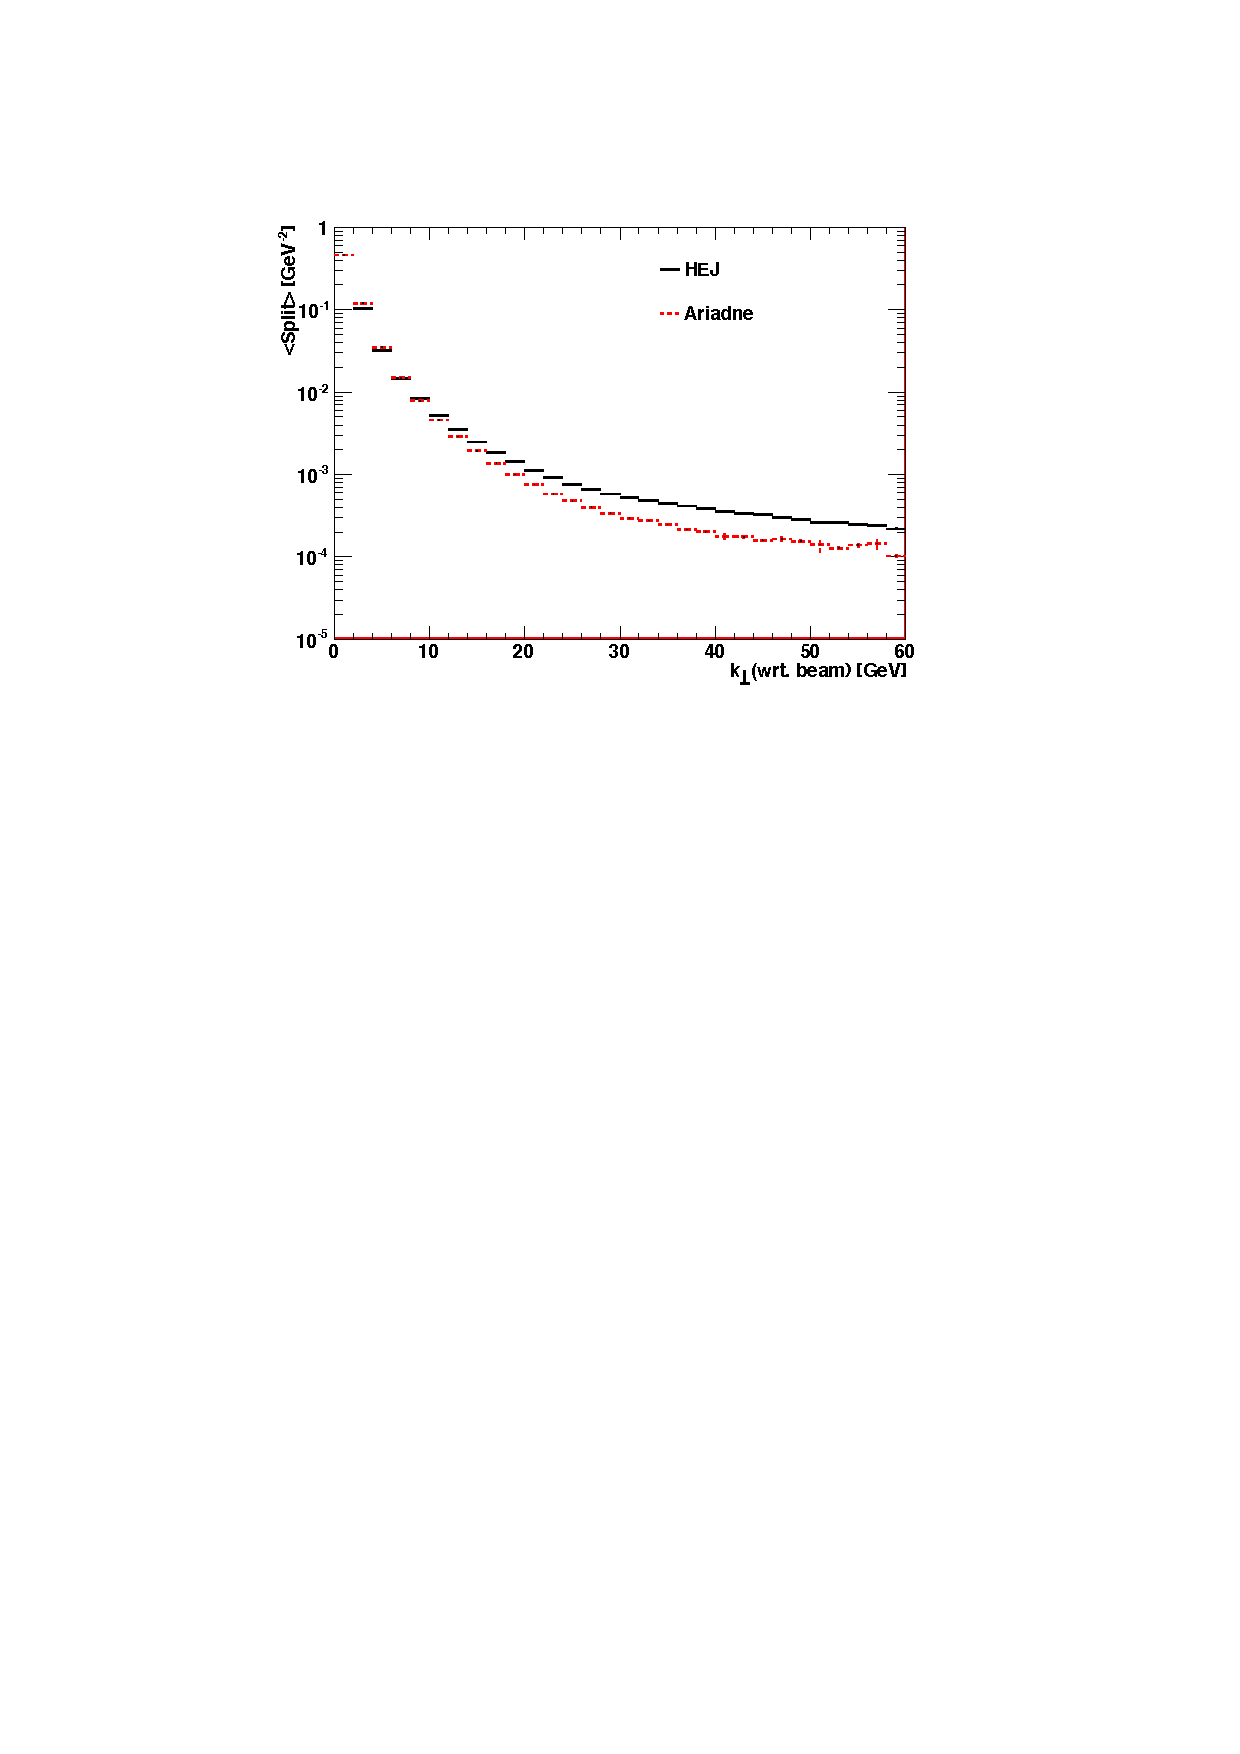
\includegraphics[width=0.75\linewidth]{heja1}
			\caption{The average splitting function for \HEJ and \ARIADNE as a function of the transverse momentum, $k_\perp$.
			Emissions are required to be well separated from the emitting parton by enforcing a cut of $\Delta r\geq0.5$
			Figure from~\cite{Andersen:2011zd}.}
			\label{fig:heja1}
		\end{figure}

		\begin{figure}[hbt]
			\centering
			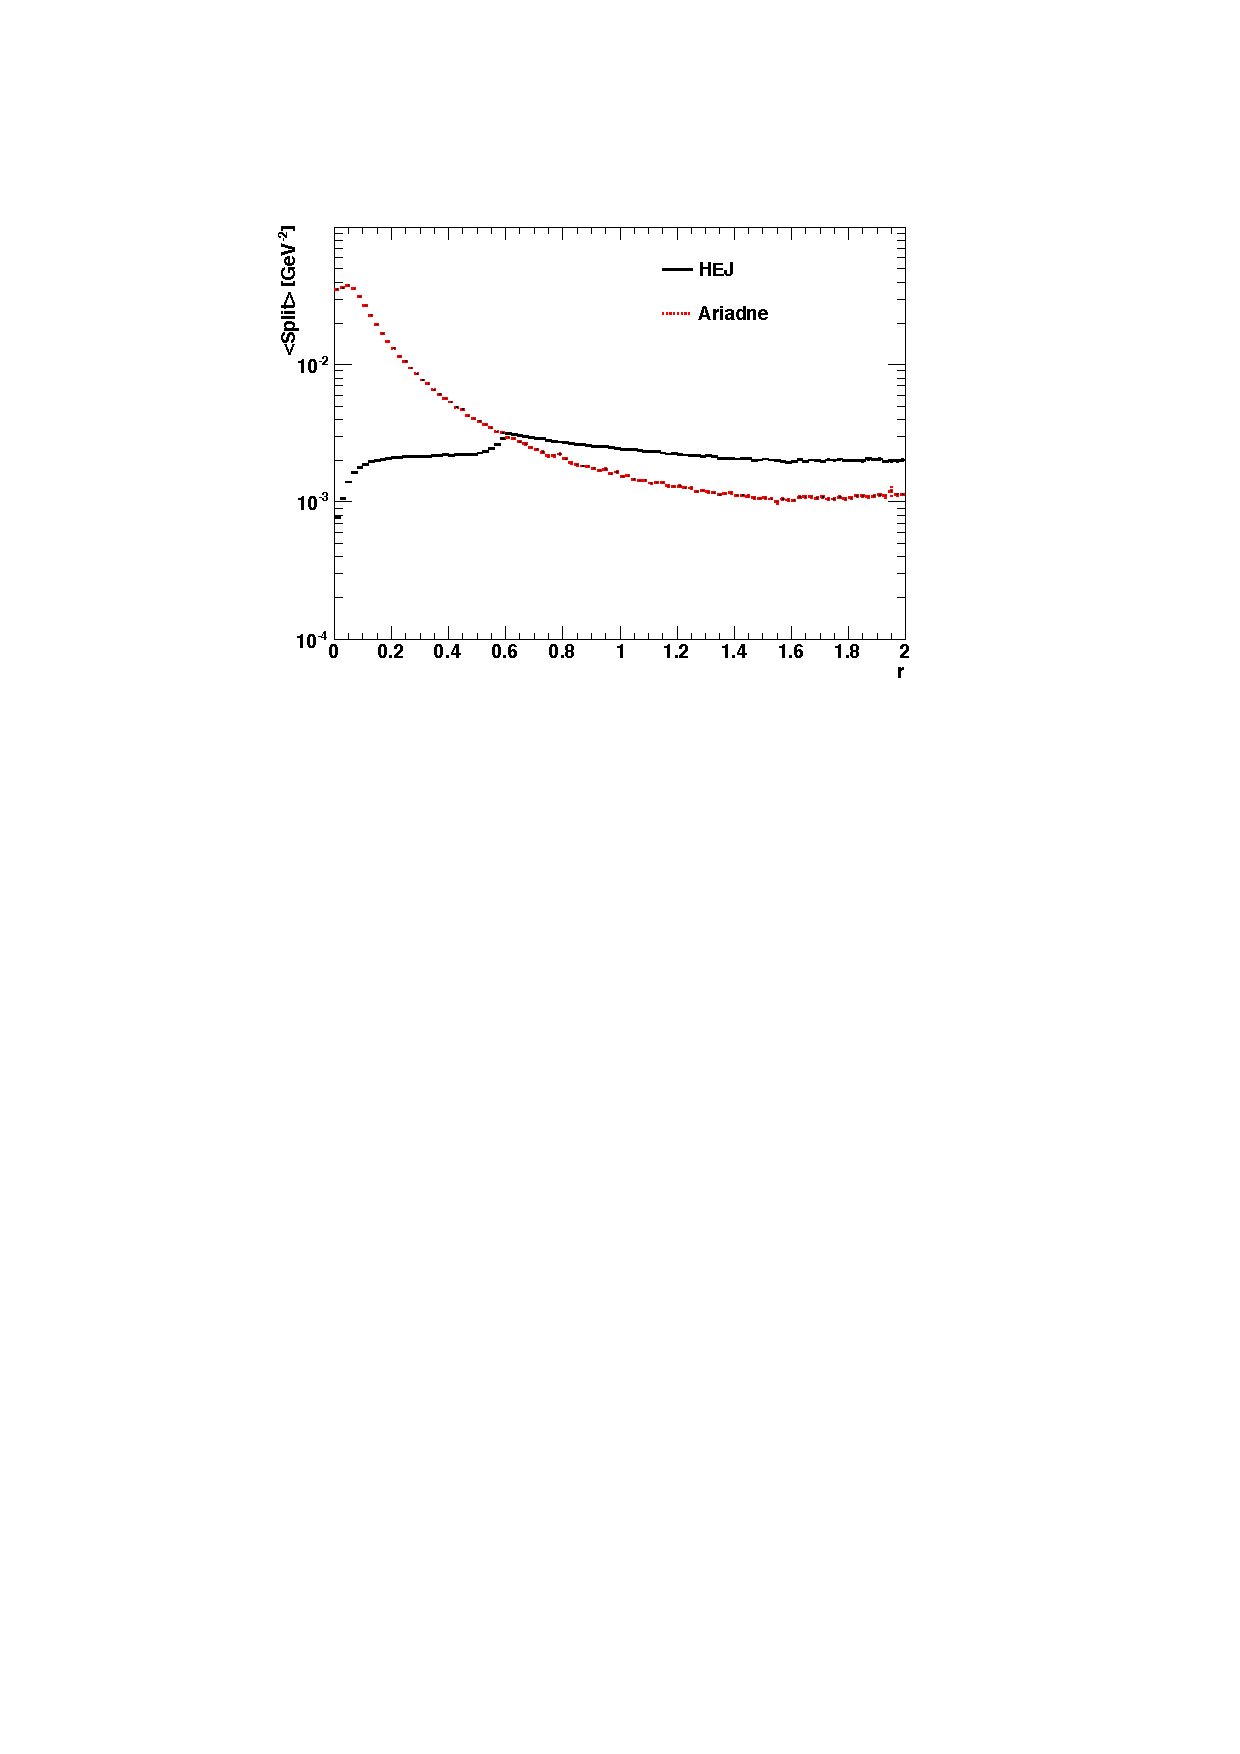
\includegraphics[width=0.75\linewidth]{heja2}
			\caption{The average splitting function for \HEJ and \ARIADNE as a function of the collinearity, $r$.
			Emissions were kept from becoming soft by enforcing a cut on the transverse momentum of $k_\perp\geq10$~GeV.
			Figure from~\cite{Andersen:2011zd}.}
			\label{fig:heja2}
		\end{figure}

	\subsection{Comparisons to data}

		The \hej framework has been thoroughly tested for a number of the currently available final states (jets,
		$W^\pm$+jets and $\zg$+jets) against other theoretical descriptions and experimental data in all of
		papers by the ATLAS, CMS and D$\emptyset$ collaborations~\cite{Aad:2011jz,Aad:2014pua,Aad:2014qxa,Aad:2014rta,
		Chatrchyan:2012gwa,Abazov:2013gpa,ZPaper}.

		These studies probe wide ranges of experimental observables with a variety of cuts designed to prove
		specific regions of phase space. \hej is seen to provide an excellent description of data in all of these
		studies in the regions of phase space close to the High Energy limit.  Interestingly there are cases where
		\HEJ is seen to be competitive with other state-of-the-art theoretical descriptions even when we are far from
		this strict limit. We now discuss a few specific examples of comparisons to data.

		In fig.~\eqref{fig:d0wjets} we see that the probability of a third emission from a dijet system (constructed
		from the most forward and backward jets in the event) in addition to a $W^\pm$ boson.  As we pull apart the
		dijet system there is increasingly more phase space into which we can radiate extra emissions and so the
		probability of emission increases.  We see that \HEJ and \texttt{BlackHat} describe the data well across
		the full range of the dijet rapidity, $\Delta y_{j_F, j_B}$, while the other generators considerably
		underestimate the dijet activity.

		Fig.~\eqref{fig:wJetsEg} describes the differential distribution for $W^\pm$ plus dijets in terms of the
		invariant mass of the dijet system defined by the two leading jets in $p_\perp$, $m_{12}$.  The logarithms
		resummed by \hej become significant for large values of $m_{12}$ and so we expect that \HEJ should
		describe this distribution well while fixed-order schemes who cannot capture these large logarithmic
		corrections may not. In fact, \HEJ gives the best description of data across almost the entire range of $m_{jj}$
		with the other theoretical predictions only agreeing with data below an invariant mass of approximately $300$~GeV
		and deviate badly by $2$~TeV.  This high invariant mass region is an important region for VBF studies and so it
		is important that we are able to describe QCD emissions here.  The failure of fixed order calculations show that
		perturbative stability already begins to breakdown in $7$~TeV LHC data.  As we will see in chapter~\ref{chap:100TeV}
		this is a challenge we must face at a potential high energy Future Circular Collider.

		\begin{figure}[hbt]
			\centering
			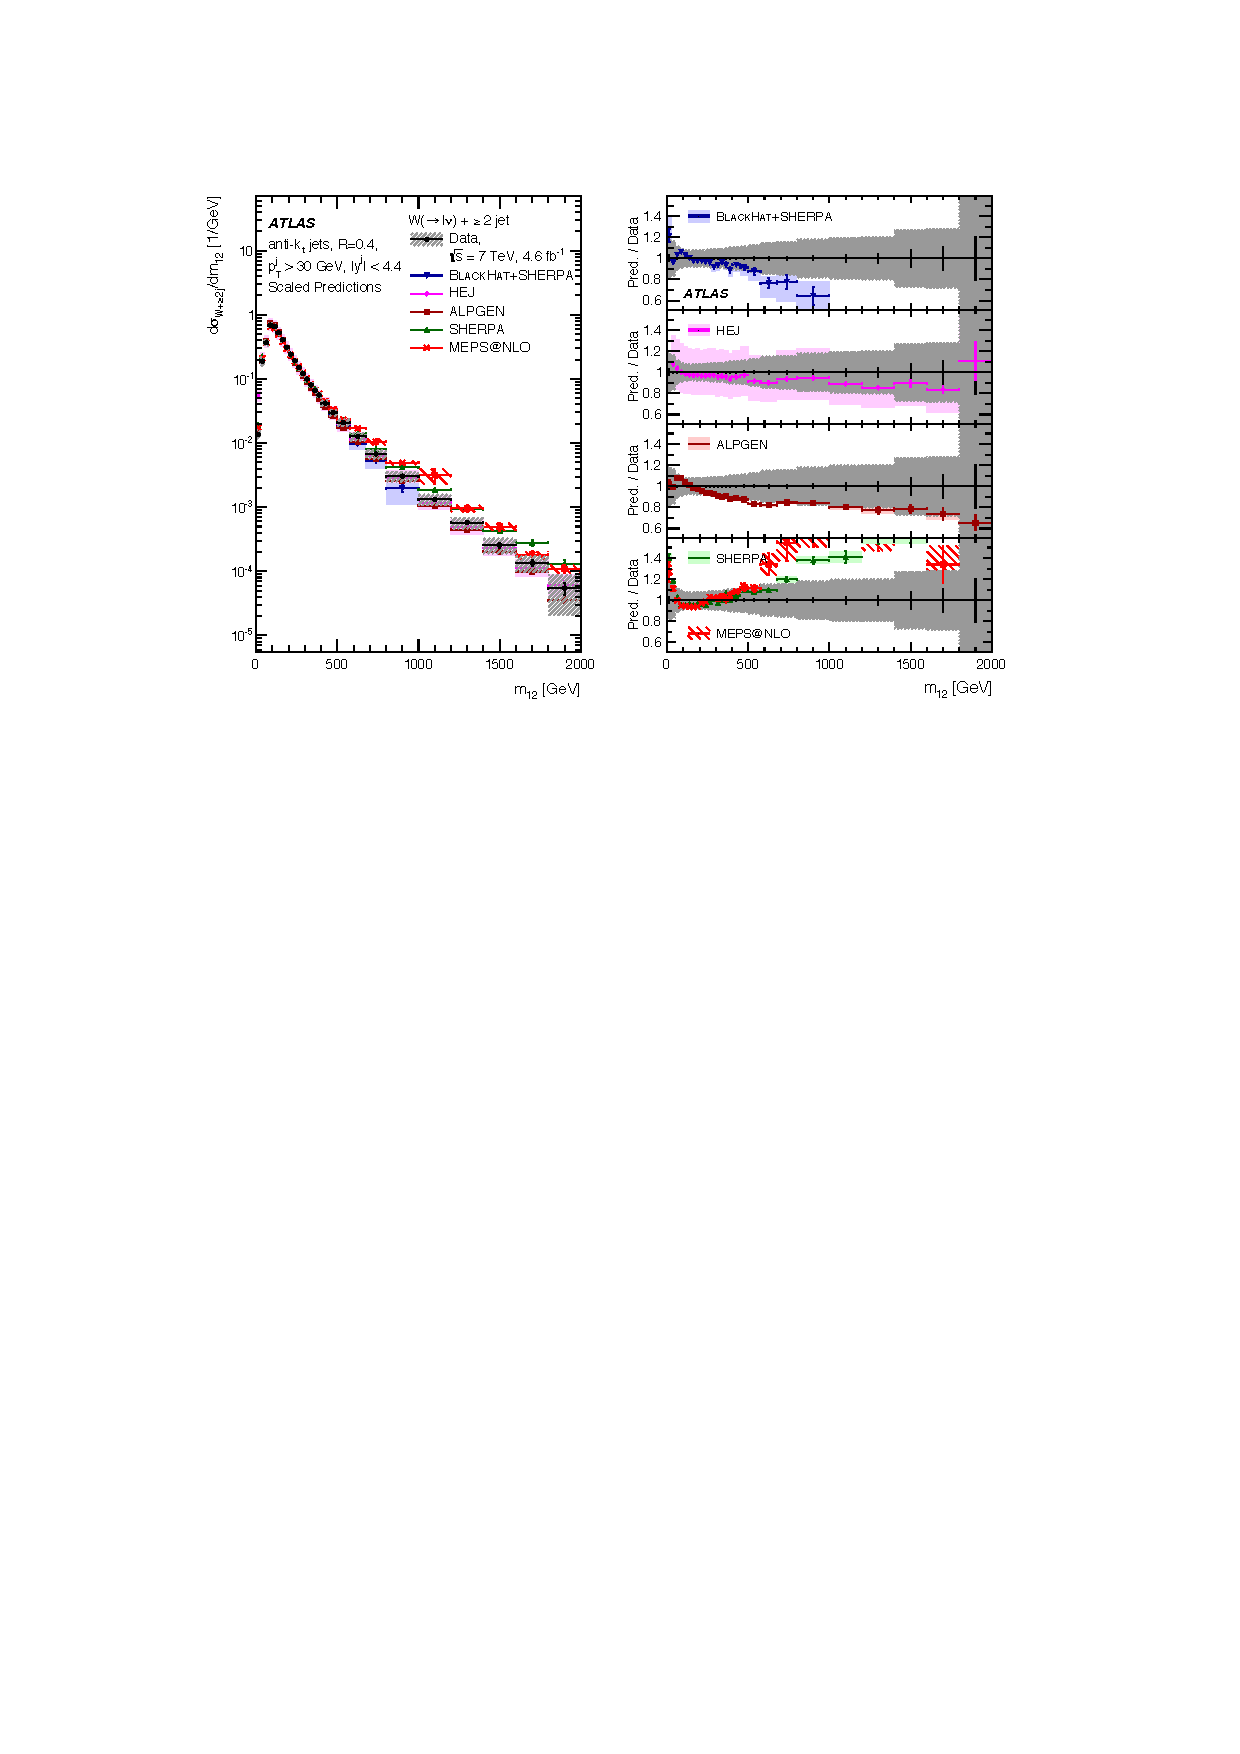
\includegraphics[width=1.0\linewidth]{wJetsEg}
			\caption{The distribution of $W^\pm$ plus inclusive dijets with at least
			2 jets differential in the invariant mass of the leading dijets in $p_\perp$, $m_{12}$.
			Fig. from \cite{Aad:2014qxa}.}
			\label{fig:wJetsEg}
		\end{figure}

